\documentclass{beamer}
%\usepackage[utf8]{inputenc}
\usepackage{textcomp}
%\usepackage{graphicx}
%\usepackage {mathtools}
%\usepackage{utopia} %font utopia imported
\usetheme{CambridgeUS}
%\usecolortheme{default}
\usepackage{minted}
%\usefonttheme{professionalfonts}
%\usepackage{natbib}
%\usepackage{hyperref}
\usepackage{colortbl}
\usepackage{pifont} % Custom bullets
%------------------------------------------------------------
% set colors
\definecolor{greyColor}{RGB}{242,242,245} % grey
\definecolor{greenColor}{RGB}{51,112,98} % green
\definecolor{yellowColor}{RGB}{246,202,84} % yellow
\definecolor{blackColor}{RGB}{84,84,84} % yellow
%------------------------------------------------------------
\setbeamercolor*{palette primary}{bg=yellowColor}
\setbeamercolor*{palette secondary}{bg=greyColor}
\setbeamercolor*{palette tertiary}{bg=greenColor, fg = white}
\setbeamercolor*{titlelike}{fg=greyColor}
\setbeamercolor*{title}{bg=greenColor, fg = white}
\setbeamercolor*{item}{fg=blackColor}
\setbeamercolor*{caption}{fg=greenColor}
\setbeamercolor{frametitle}{fg=black,bg=greyColor}

% customize the caption
\setbeamerfont{caption}{size=\footnotesize}
\setbeamercolor{caption}{fg=blackColor}
\setbeamercolor{caption name}{fg=greenColor}

% https://latex-beamer.com/tutorials/blocks/
\setbeamertemplate{blocks}[rounded][shadow=true]
\setbeamercolor{block title}{bg=greenColor, fg=white}
\setbeamercolor{block body}{bg=greyColor, fg=blackColor}

% see https://pygments.org/styles/
\usemintedstyle{solarized-light}
% [bgcolor=greyColor,linenos, breaklines,frame=leftline, numbersep=1pt,mathescape]
\setminted[shell]{bgcolor=greyColor, breaklines, numbersep=1pt,mathescape, fontsize=\footnotesize}
\setminted[rust]{bgcolor=greyColor,linenos, breaklines,frame=leftline, numbersep=1pt,mathescape, fontsize=\footnotesize}
\setminted[toml]{bgcolor=greyColor,linenos, breaklines,frame=leftline, numbersep=1pt,mathescape, fontsize=\footnotesize}
%------------------------------------------------------------
\title[Rust-Lang]{Rust Programming Language}
\author[Yumcoder]{Yumcoder}

\institute[UoT]{University of Toronto}
\date[{\today} ]
{\today}
%------------------------------------------------------------
%This block of commands puts the table of contents at the 
%beginning of each section and highlights the current section:
%\AtBeginSection[]
%{
	%  \begin{frame}
		%    \frametitle{Contents}
		%    \tableofcontents[currentsection]
		%  \end{frame}
	%}
\AtBeginSection[]{
	\begin{frame}
		\vfill
		\centering
		\begin{beamercolorbox}[sep=8pt,center,shadow=true,rounded=true]{title}
			\usebeamerfont{title}\insertsectionhead\par%
		\end{beamercolorbox}
		\vfill
	\end{frame}
}
%------------------------------------------------------------

\begin{document}
	
	%The next statement creates the title page.
	\frame{\titlepage}
	\begin{frame}
		\frametitle{Contents}
		\mbox{
			\linespread{2.3}
			\tiny
			\begin{columns}
				\column{0.5\textwidth}
				\tableofcontents[sections = 1-10]
				\column{0.5\textwidth}
				\tableofcontents[sections = 11-20]
			\end{columns}
		}
	\end{frame}
	%------------------------------------------------------------
	\section{Introduction}
	\begin{frame}[fragile]
		\frametitle{Installing rustup on Linux or macOS}
		If you’re using Linux or macOS, open a terminal and enter the following command:
		
		\inputminted{shell}{./code/install.shell}
		If the install is successful, the following line will appear:
		\begin{minted}[linenos=false, breaklines,frame=none]{shell}
			Rust is installed now. Great!
		\end{minted}
		To check whether you have Rust installed correctly, open a shell and enter this line:
		\inputminted{shell}{./code/install-check.shell}
	\end{frame}
	
	\begin{frame}[fragile]
		\frametitle{Updating, Uninstalling and Local Documentation}
		Once Rust is installed via rustup, when a new version of Rust is released, updating to the latest version is easy. From your shell, run the following update script:
		
		\inputminted{shell}{./code/install-update.shell}
		
		To uninstall Rust and rustup, run the following uninstall script from your shell:
		\inputminted{shell}{./code/install-uninstall.shell}
		
		The installation of Rust also includes a local copy of the documentation, so you can read it offline. Run \mintinline{shell}{rustup doc}  to open the local documentation in your browser.
	\end{frame}
	
	\begin{frame}[fragile]
		\frametitle{Hello, World!}
		Open a terminal and enter the following commands:
		
		\inputminted[linenos, breaklines,frame=leftline, numbersep=1pt]{shell}{./code/hello-world.shell}
		
		Make a new source file and save it as main.rs:
		\inputminted{rust}{./code/hello-world-main.rs}
		
		Compile and run the file:
		\inputminted{shell}{./code/hello-world-compile.shell}
	\end{frame}
	
	\begin{frame}[fragile]
		\frametitle{Cargo}
		\begin{itemize}
			\item Cargo is \textbf{Rust’s build system and package manager}. 
			\item Most \textbf{Rustaceans} use this tool to manage their Rust projects because Cargo handles a lot of tasks for you, such as building your code, downloading the libraries your code depends on, and building those libraries. 
			\begin{itemize}
				\item[\ding{43}] \textbf{Rustaceans} are people who use Rust, contribute to Rust, or are interested in the development of Rust.
			\end{itemize}
			\item  Cargo comes installed with Rust if you used the official installer.
			\begin{itemize}
				\item[] \inputminted{shell}{./code/cargo.shell}
			\end{itemize}
		\end{itemize}
	\end{frame}
	
	\begin{frame}[fragile]
		\frametitle{Hello, Cargo!}
		Creating a Project with Cargo:
		\inputminted{shell}{./code/hello-cargo.shell}
		
		\begin{figure}
			\centering
			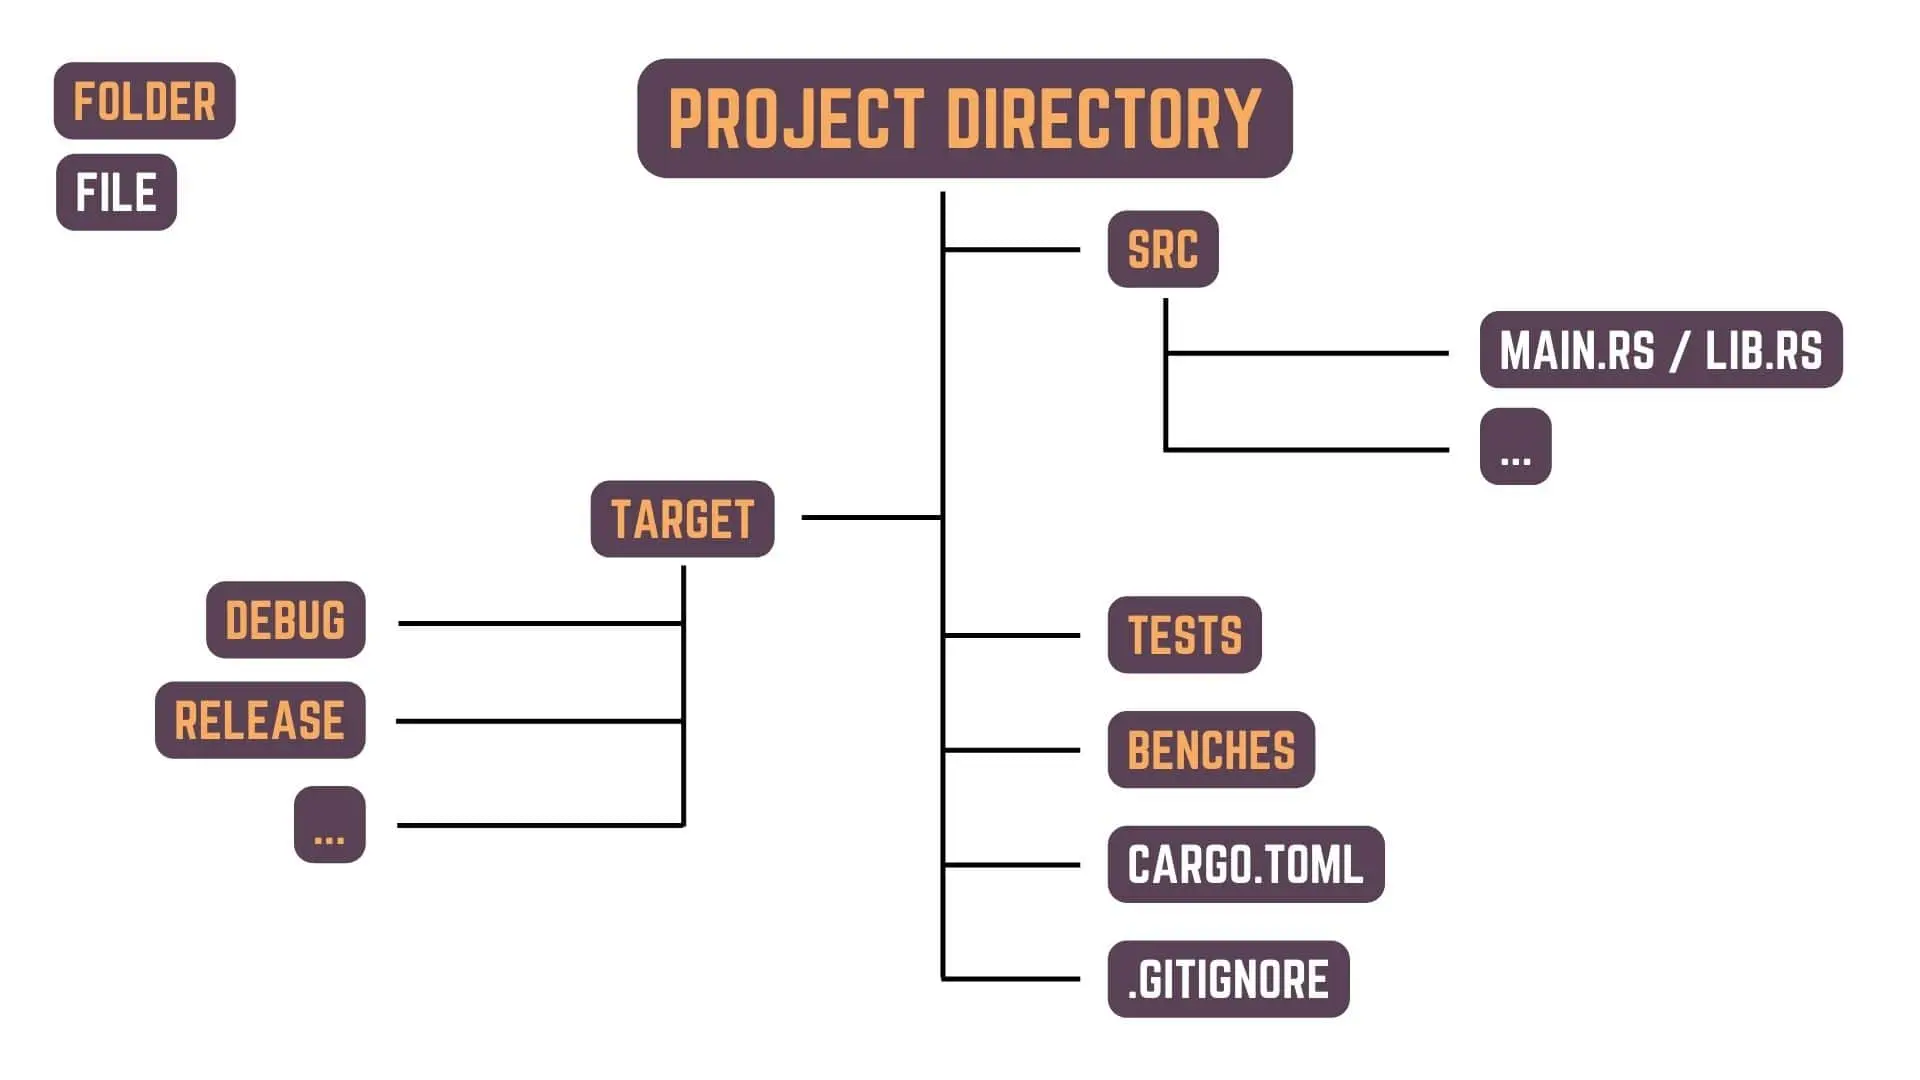
\includegraphics[width=0.65\textwidth]{./img/rust-project-folder-structure.png}
			\caption{Folder structure for projects in rust programming language.}
			\label{fig:folderRustLang}
		\end{figure}
	\end{frame}
	
	\begin{frame}[fragile]
		\frametitle{Cargo.toml}
		This file is in the \textbf{TOML} (Tom’s Obvious, Minimal Language) format, which is \textbf{Cargo’s configuration} format.
		
		\inputminted{toml}{./code/cargo.toml}
	\end{frame}
	
	\begin{frame}[fragile]
		\frametitle{Building and Running a Cargo Project}
		Now open src/main.rs and take a look:
		\inputminted{rust}{./code/hello-world-main.rs}
		
		Build your project by entering the following command:
		
		\inputminted{shell}{./code/hello-world-build.shell}
		
		\begin{itemize}
			\item Use \mintinline{shell}{cargo run} to compile and then run (all in one command).
			\item When your project is finally ready for release, you can use \mintinline{shell}{cargo build --release} to compile it with optimizations (create an executable in target/release instead of target/debug). 
		\end{itemize}
	\end{frame}
	
	\section{Common Programming Concepts}
	
	\begin{frame}{Variables and Mutability}
		\begin{itemize}
			\item by default variables are \textbf{immutable}. 
			\item This is one of many \textbf{\href{https://en.wikipedia.org/wiki/Nudge_theory}{\underline{nudges}} Rust}   gives you to write your code in a way that takes advantage of the \textbf{safety and easy concurrency }that Rust offers. 
			\begin{itemize}
				\item However, you still have the option to make your variables \textbf{mutable}. 
			\end{itemize}
		\end{itemize}
	\end{frame}
	
	\begin{frame}[fragile]
		\frametitle{Immutable variables}
		When a variable is immutable, \textit{once a value is bound to a name, you can’t change that value.}
		
		\inputminted{rust}{./code/immutable-variable.rs}
	\end{frame}
	
	\begin{frame}[fragile]
		\frametitle{Immutable variables (2)}
		You should receive an error message, as shown in this output:
		
		\inputminted{shell}{./code/immutable-variable.shell}
	\end{frame}
	
	\begin{frame}[fragile]
		\frametitle{Mutable variables}
		Although variables are immutable by default, you can make them mutable by adding \mintinline{rust}{mut} in front of the variable name.
		
		\inputminted{rust}{./code/mutable-variable.rs}
	\end{frame}
	
	\begin{frame}[fragile]
		\frametitle{Mutable variables (2)}
		\inputminted{shell}{./code/mutable-variable.shell}
	\end{frame}
	
	\begin{frame}[fragile]
		\frametitle{Constants}
		Rust’s naming convention for constants is to use \textit{all uppercase with underscores between words}.
		\inputminted[linenos=false, frame=none]{rust}{./code/const.rs}
		Like immutable variables, constants are values that are bound to a name and are not allowed to change, but there are a few differences between constants and variables.
		
		\begin{itemize}
			\item you aren’t allowed to use \mintinline{rust}{mut} with constants. Constants aren’t just immutable by default—\textbf{they’re always immutable}. You declare constants using the const keyword instead of the let keyword, and \textbf{the type of the value must be annotated}.
			
			\item 		constants may be set only to a constant expression, \textbf{not the result of a value that could only be computed at runtime}.
		\end{itemize}
	\end{frame}
	
	\begin{frame}[fragile]
		\frametitle{Shadowings}
		Rustaceans say that the first variable is shadowed by the second, which means that the second variable is what the compiler will see when you use the name of the variable.  We can shadow a variable by using the same variable’s name and repeating the use of the \mintinline{rust}{let} keyword as follows
		
		\inputminted{rust}{./code/shadowing.rs}
	\end{frame}
	
	\begin{frame}[fragile]
		\frametitle{Shadowing (2)}
		\inputminted{shell}{./code/shadowing.shell}
	\end{frame}
	
	\begin{frame}[fragile]
		\frametitle{Shadowing vs Mutable variables}
		
		We’re effectively creating a new variable when we use the let keyword again, we can change the type of the value but reuse the same name.
		
		\begin{columns}
			\column{0.5\textwidth}
			\inputminted{rust}{./code/shadowing-vs-mutable-var1.rs}
			The first spaces variable is a string type and the second spaces variable is a number type. 
			\column{0.5\textwidth}
			\inputminted{rust}{./code/shadowing-vs-mutable-var2.rs}
			we’ll get a \textbf{compile-time error}: mismatched types, expected `\&str`, found `usize`.
		\end{columns}
	\end{frame}
	
	\begin{frame}[fragile]
		\frametitle{Data Types - Primitive type}
		\begin{columns}
			\column{0.5\textwidth}
			Data type subsets: 
			\begin{itemize}
				\item Scalar
				\begin{itemize}
					\item Integers
					\item Floating-point numbers
					\item Booleans
					\item Characters
				\end{itemize}
				\item Compound
				\begin{itemize}
					\item Tuples 
					\item Arrays
				\end{itemize}
			\end{itemize}
			\column{0.5\textwidth}
			\inputminted{rust}{./code/data-types.rs}
		\end{columns}
		
		\begin{block}{Statically typed language}
			Keep in mind that Rust is a statically typed language, which means that \textbf{it must know the types of all variables at compile time}. 
		\end{block}
		
		The compiler can usually \textbf{infer} what type we want to use based on the value and how we use it (example: \mintinline{rust}{let x = 2.0; // f64}).
		
	\end{frame}
	
	\begin{frame}[fragile]
		\frametitle{Integer Types}
		\begin{itemize}
			\item An integer is a number without a fractional component.
			\item This type declaration indicates that the value it’s associated with should be an unsigned integer (signed integer types start with \textbf{i}, instead of \textbf{u}) that takes up 32 bits of space.
		\end{itemize}
		
		\begin{table}
			\begin{tabular}{|c|c|c|}
				\hline
				\rowcolor{greyColor}
				Length & Signed & Unsigned \\
				\hline
				8-bit & i8 & u8 \\
				16-bit & i16 & u16 \\
				32-bit & i32 & u32 \\
				64-bit & i64 & u64 \\
				128-bit & i128 & u128 \\
				arch\footnote{the isize and usize types depend on the architecture: 64 bits if you’re on a 64-bit architecture and 32 bits if you’re on a 32-bit architecture.} & isize & usize \\
				\hline
			\end{tabular}
		\end{table}
		
	\end{frame}
	
	\begin{frame}[fragile]
		\frametitle{Integer literals}
		\begin{itemize}
			\item A number literal is a type suffix, such as \mintinline{rust}{57u8}, to designate the type
			\item Number literals can also use \mintinline{rust}{_} as a visual separator to make the number easier to read, such as  \mintinline{rust}{1_000} , which will have the same value as if you had specified \mintinline{rust}{1000}
		\end{itemize}
		\begin{table}
			\begin{tabular}{|c|c|}
				\hline
				\rowcolor{greyColor}
				Number literals	& Example \\
				\hline
				Decimal & \mintinline{rust}{let x = 98_222} \\
				Hex & \mintinline{rust}{let x = 0xff} \\
				Octal & \mintinline{rust}{let x = 0o77} \\
				Binary & \mintinline{rust}{let x = 0b1111_0000} \\
				Byte (u8 only) & \mintinline{rust}{let x = b'A'} \\
				\hline
			\end{tabular}
		\end{table}
	\end{frame}
	
	\begin{frame}[fragile]
		\frametitle{Integer Overflow}
		\begin{itemize}
			\item Let’s say you have a variable of type u8 that can hold values between 0 and 255. 
			\item 		If you try to change the variable to a value outside of that range, such as 256, integer overflow will occur, which can result in one of two behaviors:
			\begin{itemize}
				\item When you’re compiling in \textbf{debug mode}, Rust includes checks for integer overflow that cause your program to panic at runtime if this behavior occurs.
				\item 		When you’re compiling in \textbf{release mode} with the --release flag, Rust does not include checks for integer overflow that cause panics (In the case of a u8, the value 256 becomes 0, the value 257 becomes 1, and so on).
			\end{itemize}
		\end{itemize}
	\end{frame}
	
	\begin{frame}[fragile]
		\frametitle{Floating-Point Types}
		\begin{itemize}
			
			\item Rust’s floating-point types are f32 (32 bits) and f64(64 bits), see (\href{https://en.wikipedia.org/wiki/IEEE_754}{\textsc{IEEE-754 standard}}).
			
			\item The default type is f64 because on modern CPUs it’s roughly the same speed as f32 but is capable of more precision. 
			\item All floating-point types are signed.
		\end{itemize}
		\begin{columns}
			\column{0.5\textwidth}
			\inputminted{rust}{./code/floating-types.rs}
			\column{0.5\textwidth}
			\inputminted{rust}{./code/IEEE-754.rs}
		\end{columns}
	\end{frame}
	
	\begin{frame}[fragile]
		\frametitle{Numeric Operations}
		\inputminted{rust}{./code/numeric-operations.rs}
	\end{frame}
	
	\begin{frame}[fragile]
		\frametitle{Boolean Types}
		Booleans are one byte in size.
		
		\inputminted{rust}{./code/bool-types.rs}
	\end{frame}
	
	
	\begin{frame}[fragile]
		\frametitle{Character Types}
		\begin{itemize}
			\item Note that we specify char literals with \textbf{single quotes}, as opposed to string literals, which use double quotes. 
			\item \textbf{Rust’s char type is four bytes in size} and represents a Unicode Scalar Value, which means it can represent a lot more than just ASCII.
		\end{itemize}
		\begin{figure}
			\centering
			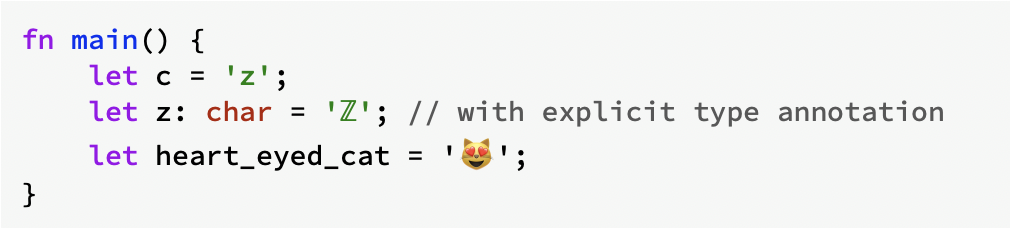
\includegraphics[width=0.65\textwidth]{./img/char.png}
		\end{figure}
	\end{frame}
	
	\begin{frame}[fragile]
		\frametitle{Tuple Types}
		A tuple is a general way of grouping together a number of values with a variety of types into one \textbf{compound type}.
		
		\inputminted{rust}{./code/tuple-types.rs}
	\end{frame}
	
	\begin{frame}[fragile]
		\frametitle{Array Types}
		\begin{itemize}
			\item Another way to have a collection of multiple values is with an array. 
			\item Unlike a tuple, every element of \textbf{an array must have the same type}. 
			\item Unlike arrays in some other languages, \textbf{arrays in Rust have a fixed length}.
			\item \textbf{Rust panics if index out of bounds}.
		\end{itemize}
		\begin{block}{Note}
			Arrays are useful when you want your data allocated on the \textbf{stack} rather than the \textbf{heap} 
		\end{block}
		
		%\inputminted{rust}{./code/tuple-types.rs}
	\end{frame}
	
	\begin{frame}[fragile]
		\frametitle{Array Types (2)}
		
		\inputminted{rust}{./code/array.rs}
	\end{frame}
	
	\begin{frame}[fragile]
		\frametitle{Functions}
		Rust code uses \textbf{snake case} as the conventional style for function and variable names, in which all letters are lowercase and underscores separate words.
		
		\inputminted{rust}{./code/function.rs}
		
		\tiny
		functions \textbf{parameters} are special variables that are part of a function’s signature. When a function has parameters, you can provide it with concrete values for those parameters. Technically, the concrete values are called \textbf{arguments}, but in casual conversation, people tend to use the words parameter and argument interchangeably.
		
	\end{frame}
	
	\begin{frame}[fragile]
		\frametitle{Statements vs Expressions}
		\begin{columns}
			\column{0.4\textwidth}
			\begin{block}{Statements}
				are instructions that perform some action and do not return a value.
			\end{block}
			\column{0.5\textwidth}
			\begin{block}{Expressions}
				evaluate to a resulting value.
			\end{block}
		\end{columns}
		\inputminted{rust}{./code/statements-expressions.rs}
	\end{frame}
	
	
	\begin{frame}[fragile]
		\frametitle{Functions with Return Values}
		\begin{itemize}
			\item Function bodies are made up of a series of statements optionally ending in an expression.
			\item Calling a function is an expression.
			\item Functions can return values to the code that calls them. 
			\item We don’t name return values, but we must declare their type after an arrow (\mintinline{rust}| ->|). 
			\item In Rust, the \textbf{return value of the function} is synonymous with \textbf{the value of the final expression in the block of the body} of a function. 
			\item You can return early from a function by using the return keyword and specifying a value, but most functions return the last expression implicitly.
		\end{itemize}
	\end{frame}
	
	\begin{frame}[fragile]
		\frametitle{Functions with Return Values (2)}
		\inputminted{rust}{./code/function-return.rs}
	\end{frame}
	
	\begin{frame}[fragile]
		\frametitle{Functions with Return Values (3)}
		\inputminted{rust}{./code/function-return2.rs}
		
		The definition of the function \mintinline{rust}|plus_one|  says that it will return an \mintinline{rust}|i32| , but statements don’t evaluate to a value, which is expressed by \mintinline{rust}|()|, the unit type.
	\end{frame}
	
	\begin{frame}[fragile]
		\frametitle{Functions with Return Values (4)}
		\inputminted{shell}{./code/function-return3.shell}
	\end{frame}
	
	\begin{frame}[fragile]
		\frametitle{if Expressions}
		if expressions are sometimes called arms
		\inputminted{rust}{./code/if.rs}
	\end{frame}
	
	\begin{frame}[fragile]
		\frametitle{if Expressions (2)}
		It’s also worth noting that the condition in this code must be a bool. If the condition isn’t a bool, we’ll get an error.
		\begin{columns}
			\column{0.5\textwidth}
			\inputminted{rust}{./code/if-err.rs}
			
			\column{0.5\textwidth}
			\inputminted{rust}{./code/if-err-correct.rs}
		\end{columns}
		\inputminted{shell}{./code/if-err.shell}
	\end{frame}
	
	\begin{frame}[fragile]
		\frametitle{Using if in a let Statement}
		Remember that blocks of code evaluate to the last expression in them, and numbers by themselves are also expressions
		\inputminted{rust}{./code/if-let.rs}
		
		The results of both the if arm and the else arm should be in the same type. So, \mintinline{rust}|let number = if condition { 5 } else { "six" };| get panic error.
	\end{frame}
	
	
	\begin{frame}[fragile]
		\frametitle{Repetition with Loops}
		The loop keyword tells Rust to execute a block of code over and over again forever or until you explicitly tell it to stop.
		\inputminted{rust}{./code/loop.rs}
	\end{frame}
	
	\begin{frame}[fragile]
		\frametitle{Returning Values from Loops}
		\inputminted{rust}{./code/loop-return.rs}
	\end{frame}
	
	\begin{frame}[fragile]
		\frametitle{Loop Labels to Disambiguate Between Multiple Loops}
		Loop labels must begin with a single quote
		\scriptsize
		\inputminted{rust}{./code/loop-label.rs}
	\end{frame}
	
	\begin{frame}[fragile]
		\frametitle{Conditional Loops with while}
		\inputminted{rust}{./code/while.rs}
	\end{frame}
	
	\begin{frame}[fragile]
		\frametitle{Repetition with for}
		\inputminted{rust}{./code/for.rs}
	\end{frame}
	
	\begin{frame}[fragile]
		\frametitle{for with range}
		\inputminted{rust}{./code/for-range.rs}
	\end{frame}
	
	\section{Understanding Ownership}
	
	\begin{frame}[fragile]
		\frametitle{What Is Ownership?}
		\begin{itemize}
			\item \textbf{Ownership} is a set of rules that governs how a Rust program manages memory.
			\item 		Some languages have \textbf{garbage collection} that \textbf{regularly looks} (performance?) for no-longer used memory as the program runs;
			\item 		 In other languages, the \textbf{programmer} must \textbf{explicitly allocate and free} the memory.
			\item 		 Rust uses a third approach: memory is managed through a system of ownership with \textbf{a set of rules} that the\textbf{ compiler checks}. If any of the rules are violated, the program won’t compile.
		\end{itemize}
		\begin{block}{Note}
			None of the features of ownership will slow down your program while it’s running.
		\end{block}
		\tiny Because ownership is a new concept for many programmers, it does take some time to get used to.
	\end{frame}
	
	
	\begin{frame}[fragile]
		\frametitle{The Stack and the Heap}
		\begin{itemize}
			\item In a systems programming language like Rust, whether a value is on the stack or the heap affects how the language behaves and why you have to make certain decisions. Parts of ownership will be described in relation to the stack and the heap later in the following, so here is a brief explanation.
			\item 	Both the \textbf{stack and the heap} are \textbf{parts of memory} available to your code to use at runtime, but they are structured in different ways. 
			\item The \textbf{stack} stores values in the order it gets them and removes the values in the opposite order. This is \textbf{referred to as last in, first out}. Adding data is called pushing onto the stack, and removing data is called popping off the stack. \textbf{All data stored on the stack must have a known, fixed size}. Data with an unknown size at compile time or a size that might change must be stored on the heap instead.
		\end{itemize}
	\end{frame}
	
	\begin{frame}[fragile]
		\frametitle{The Stack and the Heap (2)}
		\begin{itemize}
			\item 	The heap is less organized: when you put data on the heap, you request a certain amount of space. The \textbf{memory allocator} finds an empty spot in the heap that is big enough, marks it as being in use, and returns a pointer, which is the address of that location. This process is called allocating on the heap and is sometimes abbreviated as just allocating (pushing values onto the stack is not considered allocating). \textbf{Because the pointer to the heap is a known, fixed size, you can store the pointer on the stack, but when you want the actual data, you must follow the pointer}.
			\item 	\textbf{Pushing to the stack is faster than allocating on the heap} because the allocator never has to search for a place to store new data; that location is always at the top of the stack. Comparatively, allocating space on the heap requires more work, because the allocator must first find a big enough space to hold the data and then perform bookkeeping to prepare for the next allocation.
			
		\end{itemize}
	\end{frame}
	
	
	
	\begin{frame}[fragile]
		\frametitle{The Stack and the Heap (3)}
		\begin{itemize}
			\item 	When your code calls a function, the values passed into the function (including, potentially, pointers to data on the heap) and the function’s local variables get pushed onto the stack. When the function is over, those values get popped off the stack.
			\item 	Keeping track of what parts of code are using what data on the heap, minimizing the amount of duplicate data on the heap, and cleaning up unused data on the heap so you don’t run out of space are all problems that ownership addresses. Once you understand ownership, you won’t need to think about the stack and the heap very often, but knowing that the main purpose of ownership is to manage heap data can help explain why it works the way it does.
		\end{itemize}
	\end{frame}
	
	\begin{frame}[fragile]
		\frametitle{Ownership Rules}
		\begin{itemize}
			\item Each value in Rust has an owner.
			\item There can only be one owner at a time.
			\item When the owner goes out of scope, the value will be dropped.
		\end{itemize}
		
	\end{frame}
	
	\begin{frame}[fragile]
		\frametitle{Variable Scope}
		\inputminted{rust}{./code/scope.rs}
	\end{frame}
	
	\begin{frame}[fragile]
		\frametitle{The String Type}
		\begin{itemize}
			\item To illustrate the rules of ownership, we need a data type that is more complex than those we covered in the “Data Types” section
			\item The types covered previously are all a\textbf{ known size}, can be \textbf{stored on the stack and popped off the stack when their scope is over}, and can be quickly and trivially copied to make a new, independent instance if another part of code needs to use the same value in a different scope. 
			\item We want to look at \textbf{data that is stored on the heap} and explore how Rust knows when to clean up that data, and the \textbf{String} type is a great example
		\end{itemize}
	\end{frame}
	
	
	\begin{frame}[fragile]
		\frametitle{The String Type (2)}
		\begin{itemize}
			\item String literals(\mintinline{rust}|&str|) are hard-coded into our program (\textbf{fast and efficient}). String literals are convenient, but they aren’t suitable for every situation in which we may want to use text.
			\begin{itemize}
				\item 	One reason is that they’re \textbf{immutable}. 
				\item 	Another is that not every string value can be known when we write our code (for example, user input) 
			\end{itemize}
			\item 	For these situations, Rust has a second string type, \mintinline{rust}|String|.
			\begin{itemize}
				\item This type manages data allocated on the \textbf{heap} and as such is able to store an amount of text that is unknown to us at compile time.
				\item  You can create a \mintinline{rust}|String| from a string literal using the from function, like so: \mintinline{rust}|let s = String::from("hello");|.
			\end{itemize}
		\end{itemize}
	\end{frame}
	
	\begin{frame}[fragile]
		\frametitle{The String Type (3)}}
	\scriptsize
	\inputminted{rust}{./code/string.rs}
\end{frame}

\begin{frame}[fragile]
	\frametitle{Move}
	\inputminted{rust}{./code/move.rs}
	
	Bind the value 5 to x; then make a copy of the value in x and bind it to y.”  Because \textbf{integers are simple values with a known, fixed size}, and these two 5 values are pushed onto the \textbf{stack}
	
	\begin{block}{Primitive type on stack}
		\textbf{Primitive type}'s size known and fixed  so pushed onto the \textbf{stack}
	\end{block}
	
\end{frame}

\begin{frame}[fragile]
	\frametitle{Move (2)}
	
	\begin{columns}
		\column{0.6\textwidth}
		\inputminted{rust}{./code/move-string.rs}
		\column{0.4\textwidth}
		\begin{figure}
			\centering
			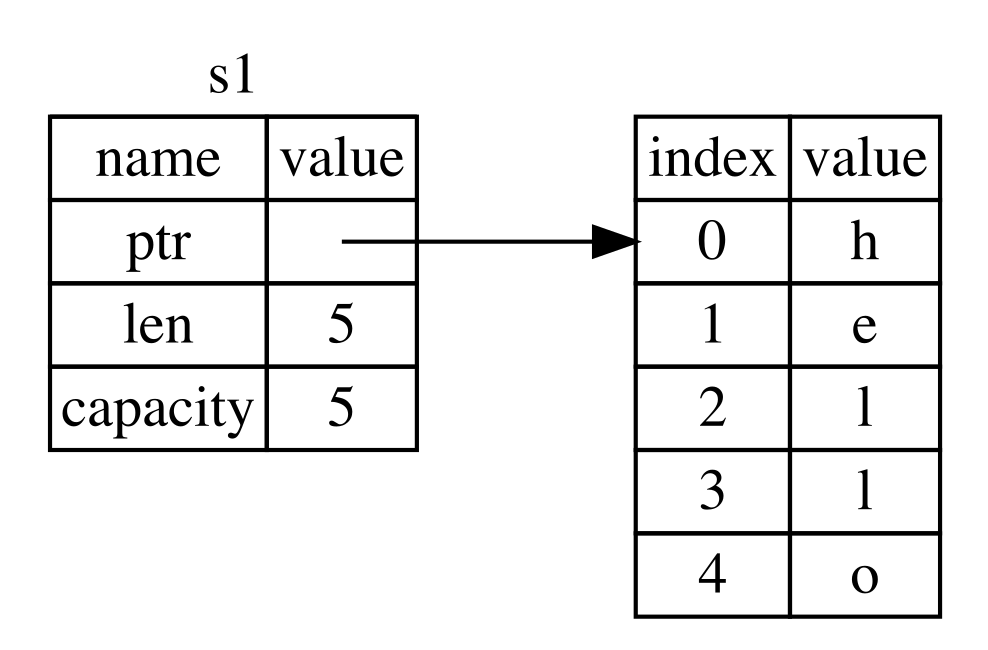
\includegraphics[width=0.65\textwidth]{./img/trpl04-01.png}
			\caption{a String in memory}
			\label{fig:figureS1}
		\end{figure}
	\end{columns}
	
	The second line would make a copy of the value in s1 and bind it to s2. But this isn’t quite what happens.
	
	\textbf{A String is made up of three parts, shown on the left: a pointer to the memory that holds the contents of the string, a length, and a capacity. This group of data is stored on the stack. On the right is the memory on the heap that holds the contents.}
\end{frame}


\begin{frame}[fragile]
	\frametitle{Move (3)}
	When we assign s1 to s2, the String data is copied, meaning we copy the pointer, the length, and the capacity that are on the stack. We do not copy the data on the heap that the pointer refers to. In other words, the data representation in memory looks like the following ( sounds like making a \textbf{shallow copy}):
	\begin{figure}
		\centering
		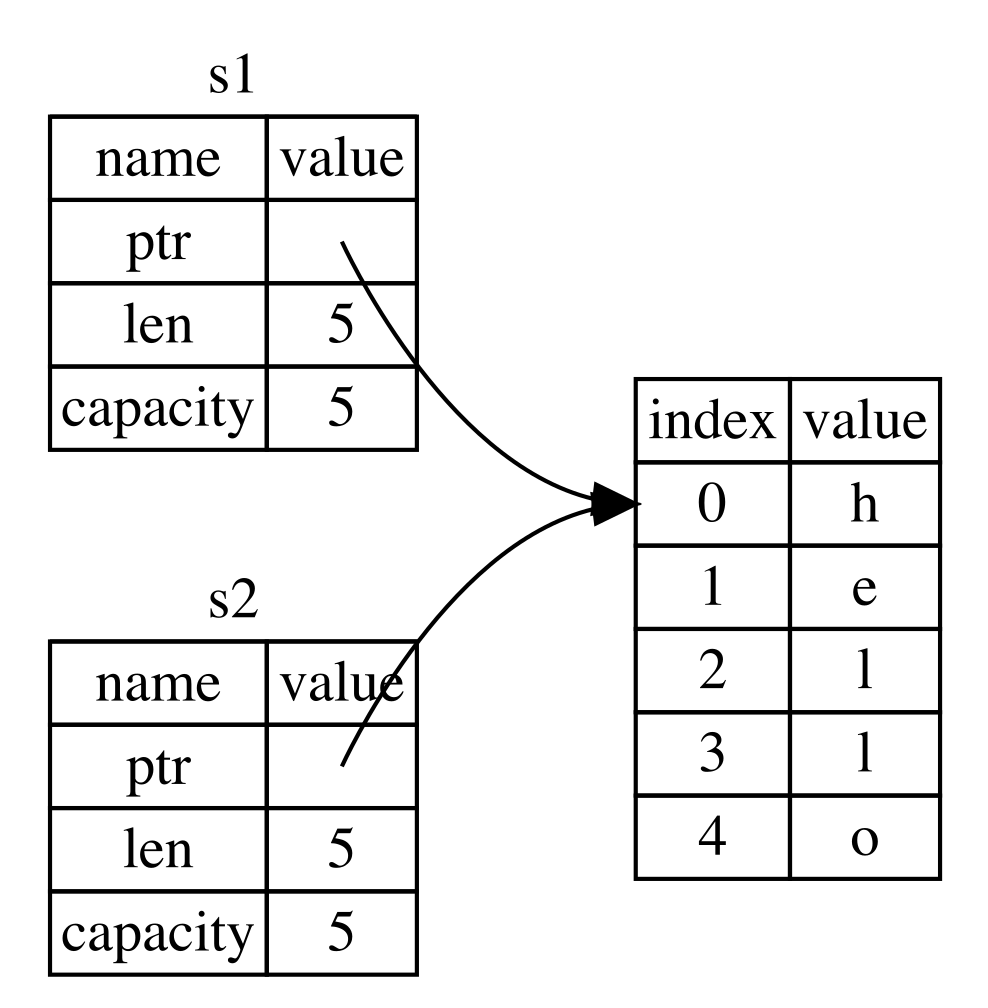
\includegraphics[width=0.3\textwidth]{./img/trpl04-02.png}
		\caption{Representation in memory of the variable s2 that has a copy of the pointer, length, and capacity of s1}
		\label{fig:figureS2}
	\end{figure}
\end{frame}



\begin{frame}[fragile]
	\frametitle{Another possibility for what s2 = s1 might do if Rust copied the heap data as well}
	The representation does not look like the following Figure, which is what memory would look like if Rust instead copied the heap data as well. If Rust did this, the operation s2 = s1 could be very expensive in terms of runtime performance if the data on the heap were large (\textbf{deep copy}).
	\begin{figure}
		\centering
		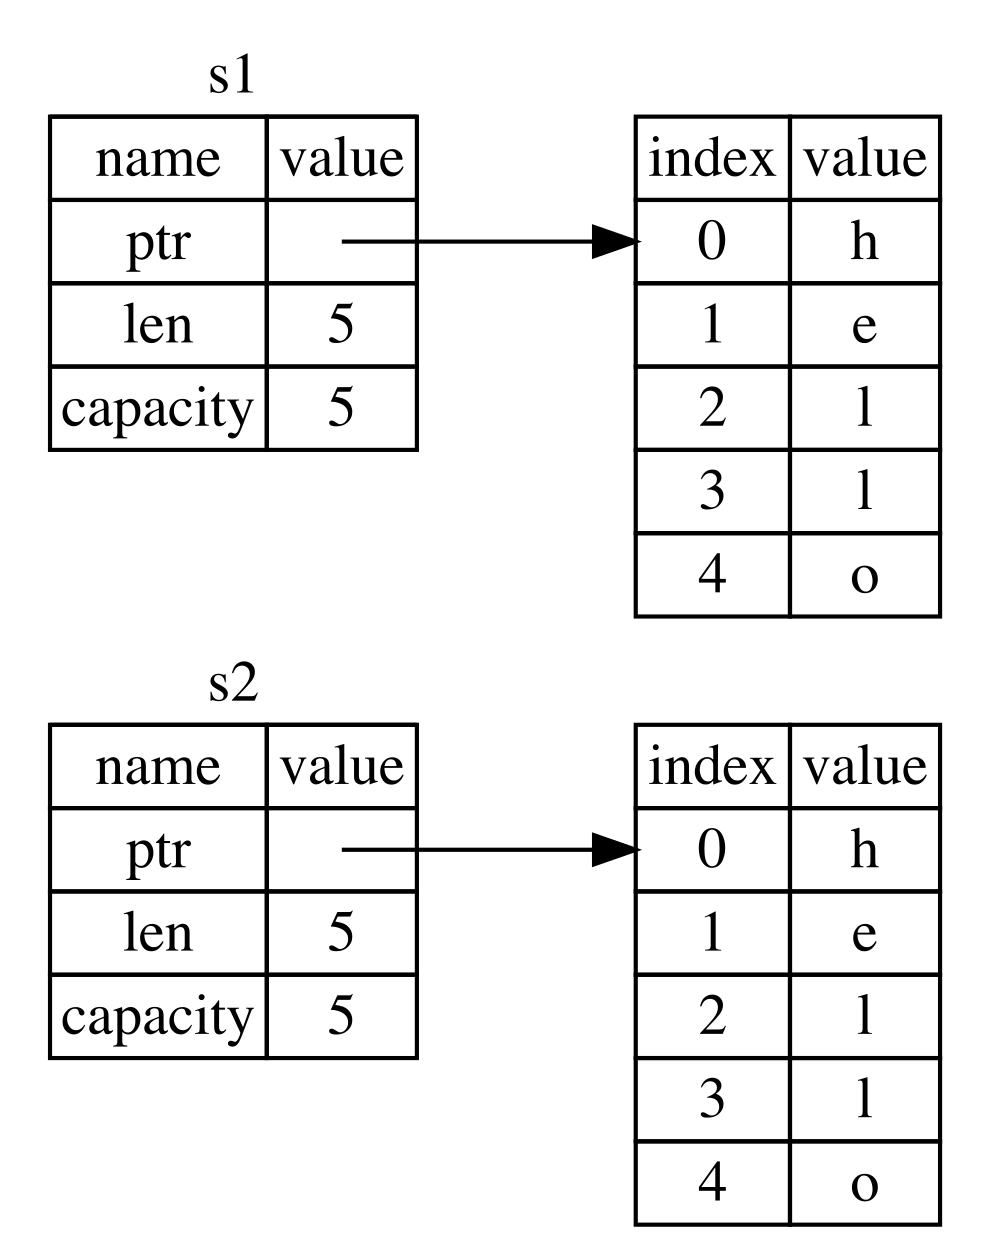
\includegraphics[width=0.3\textwidth]{./img/trpl04-03.png}
		\label{fig:figureSAnotherPossibility}
	\end{figure}
\end{frame}

\begin{frame}[fragile]
	\frametitle{s1 was moved into s2}
	\begin{itemize}
		\item When a variable goes out of scope, \textbf{Rust automatically calls the drop function and cleans up the heap memor}y for that variable. 
		\item When s2 and s1 go out of scope, they will both try to free the same memory. This is known as a \textbf{double free error} and is one of the memory safety bugs.
		\item \textbf{Freeing memory twice} can lead to memory corruption, which can potentially lead to security vulnerabilities.
		\item To ensure memory safety, after the line let s2 = s1;, Rust considers s1 as no longer valid. Therefore, Rust doesn’t need to free anything when s1 goes out of scope.
	\end{itemize}
	
\end{frame}

\begin{frame}[fragile]
	\frametitle{s1 was moved into s2 (2)}
	\inputminted{rust}{./code/move-string.rs}
\end{frame}
\begin{frame}[fragile]
	\frametitle{s1 was moved into s2 (3)}
	\inputminted{shell}{./code/move-string.shell}
\end{frame}

\begin{frame}[fragile]
	\frametitle{s1 was moved into s2 (4)}
	If you’ve heard the terms shallow copy and deep copy while working with other languages, the concept of copying the pointer, length, and capacity without copying the data probably sounds like making a shallow copy. But \textbf{because Rust also invalidates the first variable, instead of being called a shallow copy, it’s known as a move}. In this example, we would say that s1 was moved into s2. 
	\begin{figure}
		\centering
		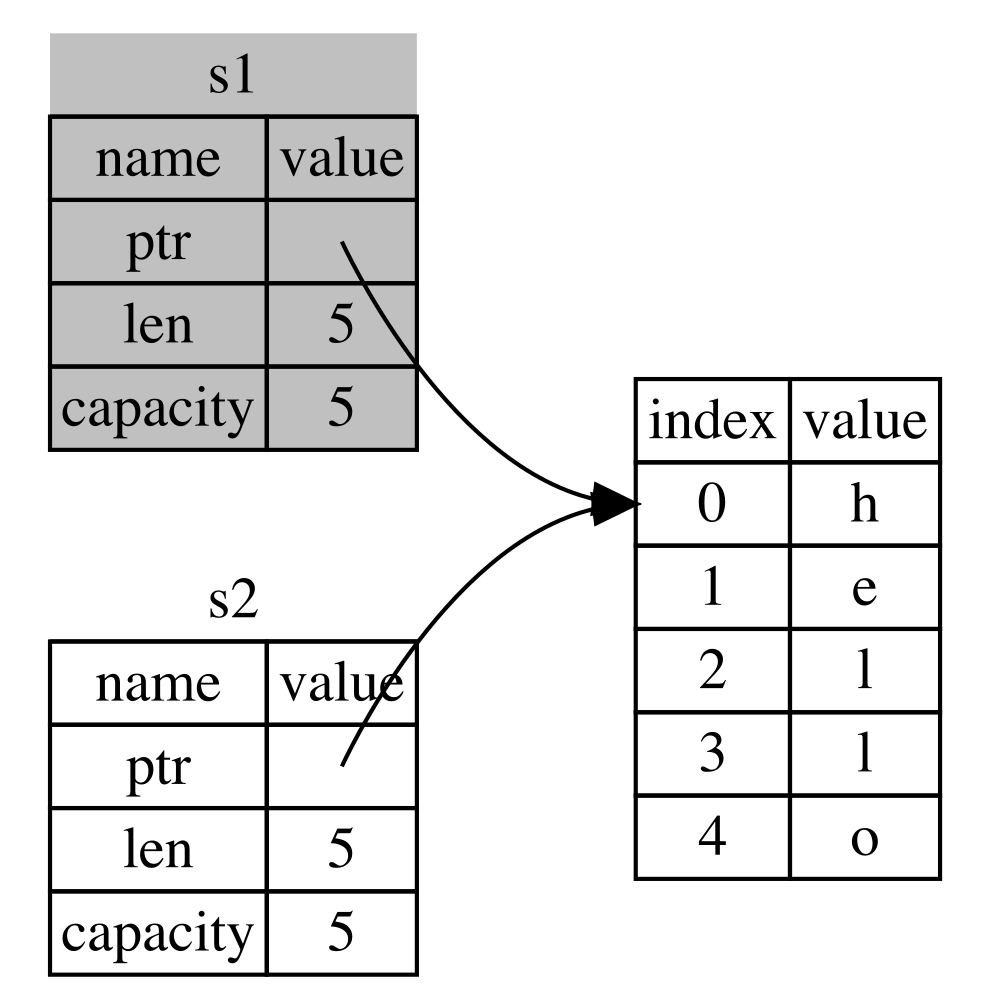
\includegraphics[width=0.3\textwidth]{./img/trpl04-04.png}
		\label{fig:figureMove}
	\end{figure}
\end{frame}

\begin{frame}[fragile]
	\frametitle{Move notes}
	
	\begin{block}{Memory safety bugs}
		That solves our problem! With only s2 valid, when it goes out of scope it alone will free the memory, and we’re done.
	\end{block}
	
	
	\begin{block}{Design choice}
		Rust will never automatically create “deep” copies of your data. Therefore, any automatic copying can be assumed to be inexpensive in terms of runtime performance.
	\end{block}
	
\end{frame}



\begin{frame}[fragile]
	\frametitle{Deeply copy with clone}
	If we do want to deeply copy the heap data of the String, not just the stack data, we can use a common method called clone.
	
	\begin{columns}
		\column{0.6\textwidth}
		\inputminted{rust}{./code/move-clone.rs}
		\column{0.4\textwidth}
		\begin{figure}
			\centering
			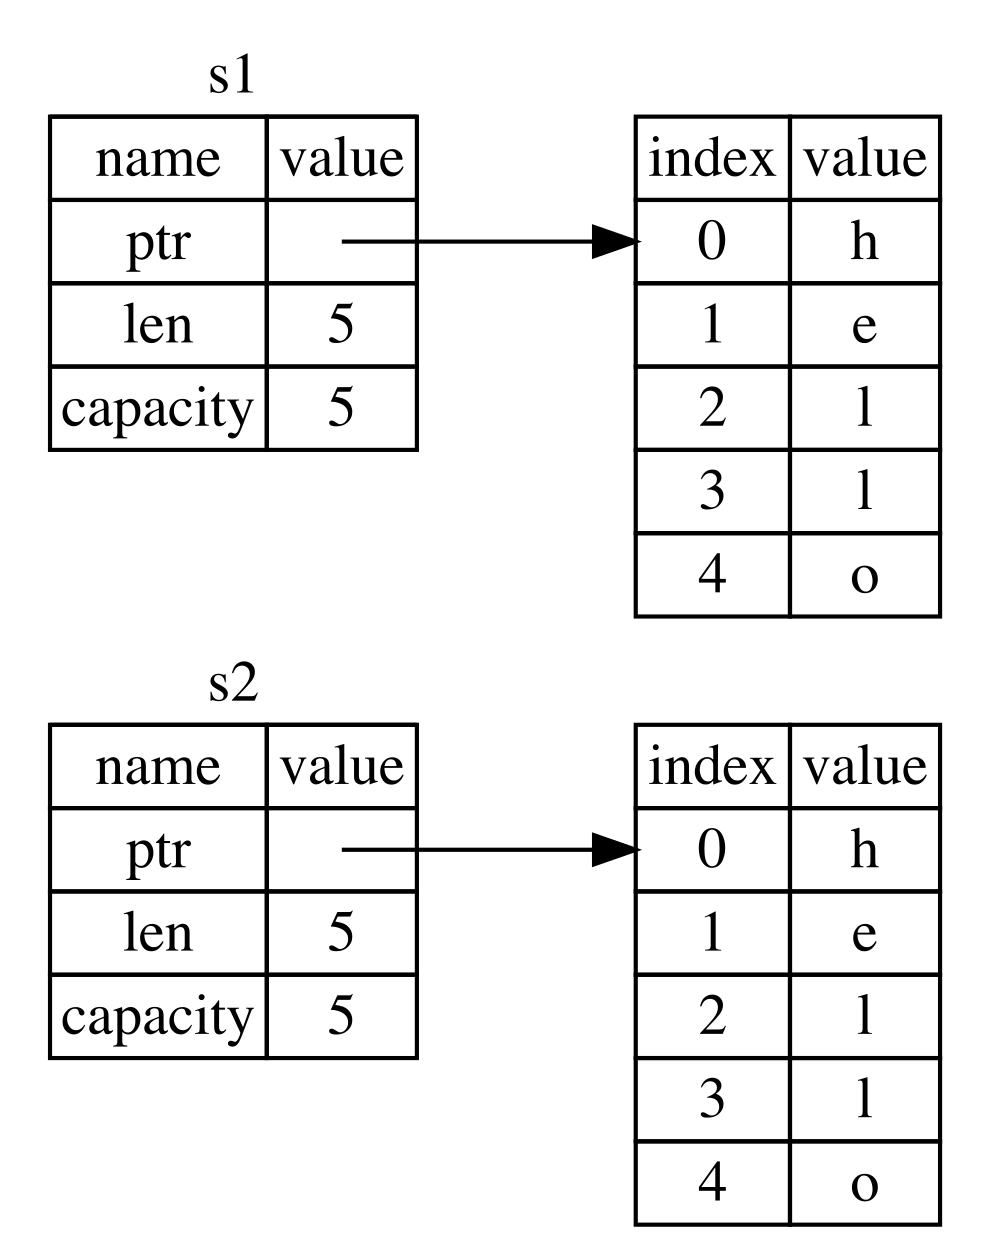
\includegraphics[width=0.8\textwidth]{./img/trpl04-03.png}
			\label{fig:figureSAnotherPossibility2}
		\end{figure}
	\end{columns}
\end{frame}



\begin{frame}[fragile]
	\frametitle{Stack-Only Data: Copy and Clone}
	We don’t have a call to clone, but x is still valid and wasn’t moved into y.
	\inputminted{rust}{./code/move2.rs}
	
	The reason is that types such as integers that have \textbf{a known size at compile time} are stored entirely on the \textbf{stack}, so \textbf{copies of the actual values are quick to make}. That means there’s no reason we would want to prevent x from being valid after we create the variable y. In other words, there’s no difference between deep and shallow copying here, so calling clone wouldn’t do anything different from the usual shallow copying, and we can leave it out.
\end{frame}

\begin{frame}[fragile]
	\frametitle{Ownership and Functions}
	\inputminted[fontsize=\scriptsize]{rust}{./code/ownership-functions.rs}
\end{frame}

\begin{frame}[fragile]
	\frametitle{Return Values and Scope}
	\inputminted[fontsize=\scriptsize]{rust}{./code/ownership-return.rs}
\end{frame}

\begin{frame}[fragile]
	\frametitle{Returning ownership}
	\inputminted{rust}{./code/ownership-return2.rs}
	Rust has a feature for using a value without transferring ownership, called \textbf{\textit{references}}.
\end{frame}

\begin{frame}[fragile]
	\frametitle{References}
	A reference is\textbf{ like a pointer} in that it’s \textbf{an address we can follow to access the data} stored at that address; \textbf{that data is owned by some other variable}. Unlike a pointer,\textbf{ a reference is guaranteed to point to a valid value of a particular type for the life of that reference}.
	\begin{columns}
		\column{0.7\textwidth}
		\inputminted[fontsize=\scriptsize]{rust}{./code/references.rs}
		\column{0.3\textwidth}
		\small
		Note that we pass \&s1 into calculate\_length and, in its definition, we take \&String rather than String. These ampersands represent references, and they allow you to refer to some value without taking ownership of it
	\end{columns}
	
\end{frame}

\begin{frame}[fragile]
	\frametitle{References (2)}
	\inputminted[fontsize=\scriptsize]{rust}{./code/references.rs}
	\begin{figure}
		\centering
		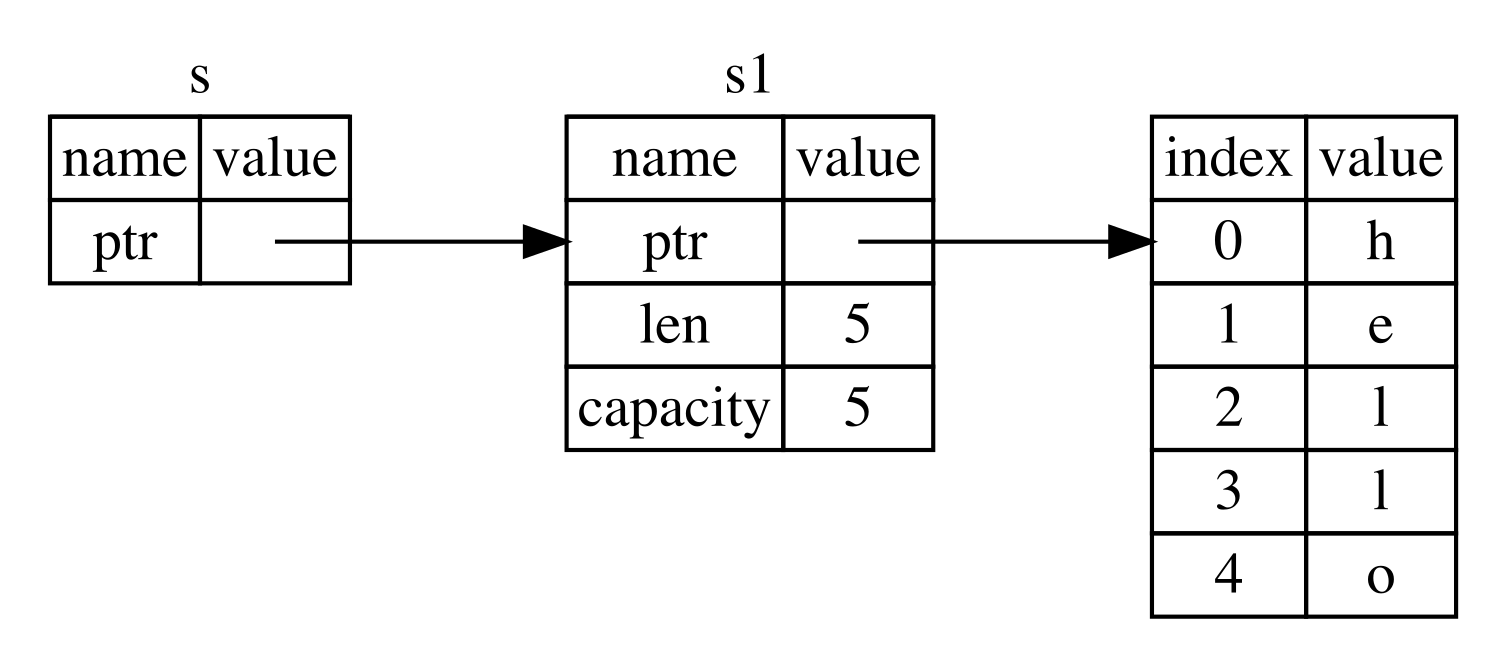
\includegraphics[width=0.6\textwidth]{./img/trpl04-05.png}
		\label{fig:figureRef}
	\end{figure}
\end{frame}

\begin{frame}[fragile]
	\frametitle{Borrowing}
	\textbf{borrowing}: \textit{the action of creating a reference}.
	As in real life, if a person owns something, you can borrow it from them. When you’re done, you have to give it back. You don’t own it. So, what happens if we try to modify something we’re borrowing?
	\inputminted{rust}{./code/borrowing.rs}
	
	\small
	Just as variables are immutable by default, so are references. We’re not allowed to modify something we have a reference to.
\end{frame}

\begin{frame}[fragile]
	\frametitle{Borrowing (2)}
	\inputminted{shell}{./code/borrowing.shell}
\end{frame}


\begin{frame}[fragile]
	\frametitle{Borrowing, Mutable References}
	We can fix the code to allow us to modify a borrowed value with just a few small tweaks that use, instead, a mutable reference (\mintinline{rust}|&mut|).
	\inputminted{rust}{./code/borrowing-mut-ref.rs}
\end{frame}


\begin{frame}[fragile]
	\frametitle{Mutable references restriction}
	\textbf{If you have a mutable reference to a value, you can have no other references to that value}. 
	\inputminted{rust}{./code/borrowing-mut-ref-err1.rs}
\end{frame}

\begin{frame}[fragile]
	\frametitle{Mutable references restriction (2)}
	\inputminted[fontsize=\scriptsize]{shell}{./code/borrowing-mut-ref-err1.shell}
	
	\scriptsize
	This error says that this code is invalid because we cannot borrow s as mutable more than once at a time. The first mutable borrow is in r1 and must last until it’s used in the println!, but between the creation of that mutable reference and its usage, we tried to create another mutable reference in r2 that borrows the same data as r1.
	
\end{frame}

\begin{frame}[fragile]
	\frametitle{Why mutable references restriction exist in Rust?}
	It’s something that new Rustaceans struggle with because most languages let you mutate whenever you’d like. The benefit of having this restriction is that \textbf{Rust can prevent data races at compile time}. 
	
	A data race is similar to a race condition and happens when these three behaviors occur:
	
	\begin{itemize}
		\item Two or more pointers access the same data at the same time.
		\item 	At least one of the pointers is being used to write to the data.
		\item 	There’s no mechanism being used to synchronize access to the data.
	\end{itemize}
	Data races cause undefined behavior and can be difficult to diagnose and fix when you’re trying to track them down at runtime.
	
\end{frame}


\begin{frame}[fragile]
	\frametitle{Mutable references restriction example}
	As always, we can use curly brackets to create a new scope, allowing for multiple mutable references, just not simultaneous ones:
	\inputminted{rust}{./code/borrowing-simultaneous.rs}
\end{frame}

\begin{frame}[fragile]
	\frametitle{Mutable references restriction example (combining mutable and immutable references)}
	\inputminted{rust}{./code/borrowing-combining.rs}
\end{frame}

\begin{frame}[fragile]
	\frametitle{Mutable references restriction example (combining mutable and immutable references)}
	\inputminted{shell}{./code/borrowing-combining.shell}
\end{frame}

\begin{frame}[fragile]
	\frametitle{Mutable references restriction example (combining mutable and immutable references, note to  reference’s scope)}
	\inputminted{rust}{./code/borrowing-combining-note.rs}
\end{frame}

\begin{frame}[fragile]
	\frametitle{Dangling References}
	In languages with pointers, it’s easy to erroneously create a dangling pointer—\textbf{a pointer that references a location in memory that may have been given to someone else}—by freeing some memory while preserving a pointer to that memory. In Rust, by contrast, \textbf{the compiler guarantees that references will never be dangling references}: if you have a reference to some data, the compiler will ensure that the data will not go out of scope before the reference to the data does.
	\inputminted[fontsize=\scriptsize]{rust}{./code/dangling.rs}
\end{frame}

\begin{frame}[fragile]
	\frametitle{Dangling References (2)}
	
	\inputminted{shell}{./code/dangling.shell}
\end{frame}

\begin{frame}[fragile]
	\frametitle{Dangling References (3), solution}
	The solution here is to return the String directly:
	
	\inputminted{rust}{./code/dangling-sol.rs}
	
	This works without any problems. \textbf{Ownership is moved out, and nothing is deallocated.}
\end{frame}


\begin{frame}[fragile]
	\frametitle{The Slice Type}
	\textbf{Slices} let you \textbf{reference a contiguous sequence of elements in a collection} rather than the whole collection. A slice is \textbf{a kind of reference, so it does not have ownership}.
\end{frame}

\begin{frame}[fragile]
	\frametitle{Learn application of Slice Type by example}
	Here’s a small programming problem: write a function that takes a string of words separated by spaces and returns the first word it finds in that string.
	\scriptsize
	\inputminted[fontsize=\scriptsize]{rust}{./code/slice.rs}
\end{frame}

\begin{frame}[fragile]
	\frametitle{Learn application of Slice Type by example}
	\begin{itemize}
		\item This program compiles without any errors and would also do so if we used word after calling s.clear(). Because word isn’t connected to the state of s at all, word still contains the value 5. We could use that value 5 with the variable s to try to extract the first word out, but this would be a bug because the contents of s have changed since we saved 5 in word.
		\item Luckily, Rust has a solution to this problem: string slices.
	\end{itemize}
\end{frame}

\begin{frame}[fragile]
	\frametitle{String Slices}
	
	\begin{columns}
		\column{0.6\textwidth}
		\inputminted{rust}{./code/string-slice.rs}
		\column{0.4\textwidth}
		\begin{figure}
			\centering
			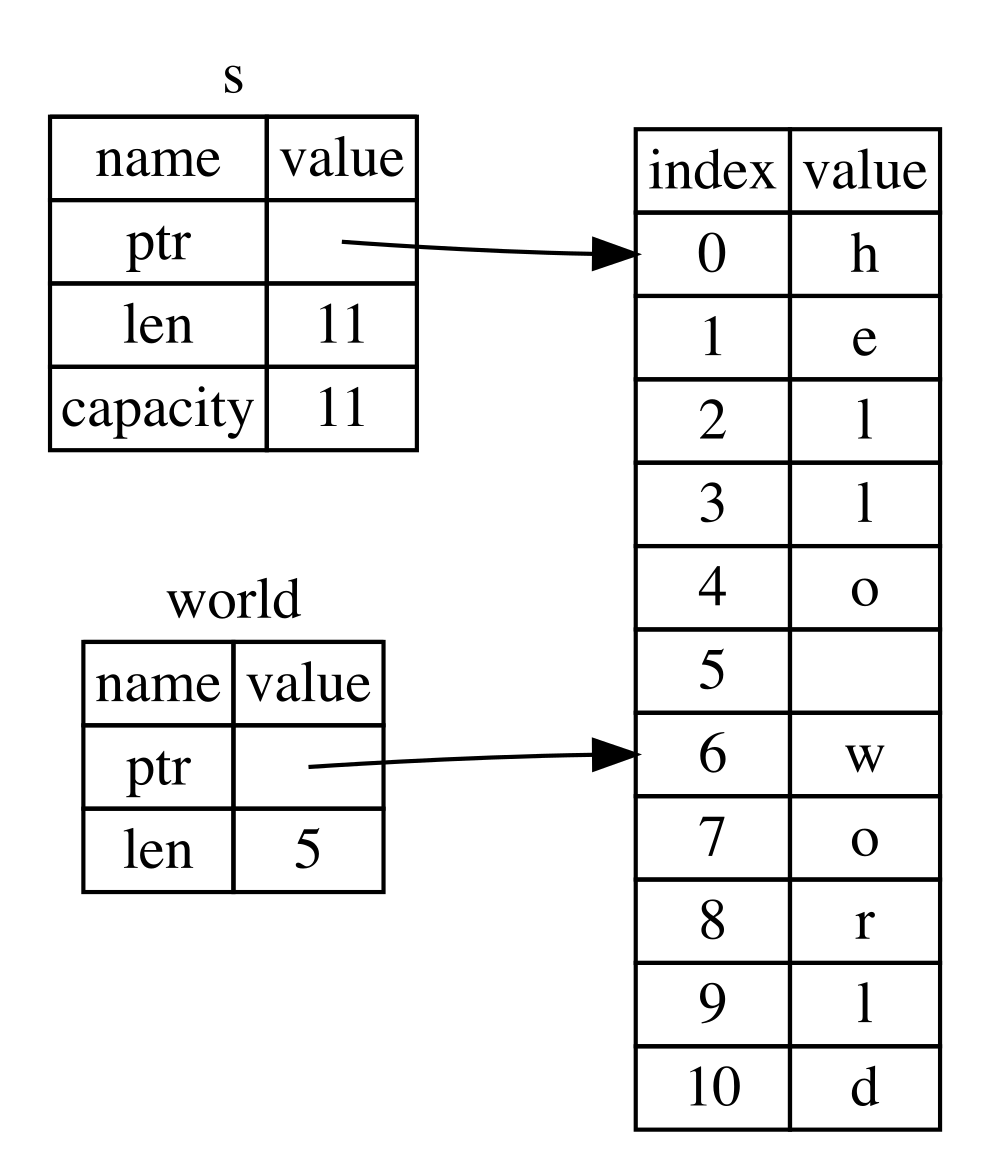
\includegraphics[width=0.8\textwidth]{./img/trpl04-06.png}
		\end{figure}
		
	\end{columns}
	
\end{frame}

\begin{frame}[fragile]
	\frametitle{Rewrite first\_word to return a slice}
	\inputminted{rust}{./code/slice2.rs}
\end{frame}

\begin{frame}[fragile]
	\frametitle{ Rewrite first\_word to return a slice (2)}
	\inputminted{shell}{./code/slice2.shell}
\end{frame}

\begin{frame}[fragile]
	\frametitle{Rewrite first\_word to return a slice (3)}
	Recall from the borrowing rules that if we have an immutable reference to something, we cannot also take a mutable reference. Because clear needs to truncate the String, it needs to get a mutable reference. The println! after the call to clear uses the reference in word, so the immutable reference must still be active at that point. Rust disallows the mutable reference in clear and the immutable reference in word from existing at the same time, and compilation fails. Not only has Rust made our API easier to use, but it has also eliminated an entire class of errors at compile time!
\end{frame}

\begin{frame}[fragile]
	\frametitle{Improve first\_word function}
	\mintinline{rust}|fn first_word(s: &String) -> &str {/*...*/}| 
	
	A more experienced Rustacean would write the signature as in below instead because it allows us to use the same function on both \mintinline{rust}|&String|  values and  \mintinline{rust}|&str|  values.
	
	\mintinline{rust}|fn first_word(s: &str) -> &str {/*...*/}| 
\end{frame}


\section{Using Structs to Structure Related Data}

\begin{frame}[fragile]
	\frametitle{Defining and Instantiating Structs}
	\begin{itemize}
		\item A\textbf{ struct, or structure,} is a custom data type that lets you package together and name multiple related values that make up a meaningful group. If you’re familiar with an object-oriented language, a struct is like an\textit{ object’s data attributes}.
		\item 	\textbf{Structs are similar to tuples}, in that both hold multiple related values. Like tuples, the pieces of a struct can be different types. Unlike with tuples, in a struct you’ll name each piece of data so it’s clear what the values mean. Adding these names means that structs are more flexible than tuples: you don’t have to rely on the order of the data to specify or access the values of an instance.
	\end{itemize}
\end{frame}

\begin{frame}[fragile]
	\frametitle{Defining and Instantiating Structs (2)}
	\inputminted{rust}{./code/struct.rs}
\end{frame}

\begin{frame}[fragile]
	\frametitle{Using the Field Init Shorthand}
	\inputminted{rust}{./code/field-shorthand.rs}
\end{frame}

\begin{frame}[fragile]
	\frametitle{Creating Instances From Other Instances With Struct Update Syntax}
	\inputminted{rust}{./code/struct-build.rs}
\end{frame}

\begin{frame}[fragile]
	\frametitle{Creating Instances From Other Instances With Struct Update Syntax (2)}
	The ..user1 \textbf{must come last to specify that any remaining fields should get their values from the corresponding fields} in user1.
	
	\begin{block}{Note that the struct update syntax uses = like an assignment}
		This is because it moves the data. In this example, we can no longer use user1 after creating user2 because the String in the username field of user1 was moved into user2. If we had given user2 new String values for both email and username, and thus only used the active and sign\_in\_count values from user1, then user1 would still be valid after creating user2. The types of active and sign\_in\_count are types that implement the Copy trait.
	\end{block}
	
\end{frame}


\begin{frame}[fragile]
	\frametitle{Creating Instances From Other Instances With Struct Update Syntax (3)}
	\inputminted{rust}{./code/struct-err.rs}
\end{frame}


\begin{frame}[fragile]
	\frametitle{Creating Instances From Other Instances With Struct Update Syntax (4)}
	\inputminted{shell}{./code/struct-err2.shell}
\end{frame}

\begin{frame}[fragile]
	\frametitle{Ownership of Struct Data}
	\begin{itemize}
		\item In the User struct definition,\textbf{ we used the owned String type rather than the \mintinline{rust}|&str| string slice type.} This is a deliberate choice because we want each instance of this struct to own all of its data and for that data to be valid for as long as the entire struct is valid.
		\item 	\textbf{It’s also possible for structs to store references to data owned by something else, but to do so requires the use of lifetimes}, a Rust feature that we’ll discuss later. Lifetimes ensure that the data referenced by a struct is valid for as long as the struct is.
	\end{itemize}
\end{frame}


\begin{frame}[fragile]
	\frametitle{Using Tuple Structs without Named Fields to Create Different Types}
	Rust also supports structs that look similar to tuples, called tuple structs. Tuple structs have the added meaning the struct name provides but don’t have names associated with their fields; rather, they just have the types of the fields. Tuple structs are useful when you want to give the whole tuple a name and make the tuple a different type from other tuples, and when naming each field as in a regular struct would be verbose or redundant.
	\inputminted{rust}{./code/tuple-struct.rs}
\end{frame}


\begin{frame}[fragile]
	\frametitle{Unit-Like Structs Without Any Fields}
	You can also define structs that don’t have any fields! These are called \textbf{unit-like structs} because they behave similarly to ().
	\inputminted{rust}{./code/unit-like-struct.rs}
	
	\begin{block}{Unit type}
		The tuple without any values has a special name, unit. This value and its corresponding type are both written () and represent an empty value or an empty return type. Expressions implicitly return the unit value if they don’t return any other value.
	\end{block}
\end{frame}

\begin{frame}[fragile]
	\frametitle{Unit-Like Structs Without Any Fields (2)}
	Unit-like structs can be useful when you need to implement a trait on some type but don’t have any data that you want to store in the type itself. 
	Example, see: The global memory allocator, \href{https://doc.rust-lang.org/src/alloc/alloc.rs.html#59}{\colorbox{lightgray}{Global}}, is a unit struct.
\end{frame}

\begin{frame}[fragile]
	\frametitle{Method Syntax}
	\textbf{Methods} are similar to \textbf{functions}: we declare them with the \mintinline{rust}|fn| keyword and a name, they can have parameters and a return value, and they contain some code that’s run when the method is called from somewhere else. Unlike functions, methods are defined within the context of a struct (or an enum or a trait object, which we cover later), and their \textbf{first parameter is always self}, which represents the instance of the struct the method is being called on.
\end{frame}

\begin{frame}[fragile]
	\frametitle{Method Syntax(2)}
	\inputminted{rust}{./code/method.rs}
\end{frame}

\begin{frame}[fragile]
	\frametitle{Associated Functions}
	\begin{itemize}
		\item \textbf{All functions defined within an \mintinline{rust}|impl|  block} are called associated functions because they’re associated with the type named after the  \mintinline{rust}|impl| . We can define associated functions that don’t have self as their first parameter (and\underline{ thus are not methods}) because they don’t need an instance of the type to work with. We’ve already used one function like this: the String::from function that’s defined on the String type.
		\item 	Associated functions that aren’t methods are often used for constructors that will return \textbf{a new instance of the struct}(factory method). These are often called \textbf{new}, but new isn’t a special name and isn’t built into the language.
	\end{itemize}
\end{frame}

\begin{frame}[fragile]
	\frametitle{Associated Functions}
	\inputminted{rust}{./code/factory-method.rs}
\end{frame}

\begin{frame}[fragile]
	\frametitle{Multiple \mintinline{rust}|impl| Blocks}
	\inputminted{rust}{./code/multi-impl.rs}
\end{frame}

\section{Enums and Pattern Matching}
\begin{frame}[fragile]
	\frametitle{Defining an Enum}
	Enums allow you to define a type by enumerating its possible variants.
	\begin{block}{Struct vs Enum}
		Where structs give you a way of grouping together related fields and data, like a Rectangle with its width and height, enums give you a way of saying a value is one of a possible set of values. 
	\end{block}
	\inputminted{rust}{./code/enum.rs}
\end{frame}

\begin{frame}[fragile]
	\frametitle{Defining an Enum (2)}
	There’s another advantage to using an enum rather than a struct:\textbf{ each variant can have different types and amounts of associated data}. 
	\inputminted{rust}{./code/enum2.rs}
\end{frame}

\begin{frame}[fragile]
	\frametitle{Defining an Enum (3)}
	
	\inputminted{rust}{./code/enum3.rs}
\end{frame}

\begin{frame}[fragile]
	\frametitle{The Option Enum and Its Advantages Over Null Values}
	The Option type encodes the very common scenario in which a value could be something or it could be nothing.
	\inputminted{rust}{./code/enum4.rs}
	
	see: “Null References: The Billion Dollar Mistake”
\end{frame}

\begin{frame}[fragile]
	\frametitle{Advantage of Option Over Null}
	\begin{itemize}
		\item 	When we have a Some value, we know that a value is present and the value is held within the Some. When we have a None value, in some sense, it means the same thing as null: we don’t have a valid value. So why is having \mintinline{rust}|Option<T>| any better than having null?
		\begin{itemize}
			\item 	In short, because \mintinline{rust}|Option<T>| and T (where T can be any type) are different types, the compiler won’t let us use an \mintinline{rust}|Option<T>| value as if it were definitely a valid value. For example, this code won’t compile because it’s trying to add an \mintinline{rust}|i8| to an \mintinline{rust}|Option<i8>|:
		\end{itemize}
	\end{itemize}
	
	\inputminted{rust}{./code/enum5.rs}
\end{frame}

\begin{frame}[fragile]
	\frametitle{The match Control Flow Construct}
	Rust has an extremely powerful control flow construct called \mintinline{rust}|match| that allows you to compare a value against a series of patterns and then execute code based on which pattern matches.
	\inputminted{rust}{./code/match.rs}
\end{frame}

\begin{frame}[fragile]
	\frametitle{Patterns that Bind to Values}
	\begin{columns}
		\column{0.8\textwidth}
		\inputminted[fontsize=\scriptsize]{rust}{./code/match2.rs}
		\column{0.2\textwidth}
		Another useful feature of match arms is that they can bind to the parts of the values that match the pattern. This is how we can extract values out of enum variants.
	\end{columns}
\end{frame}

\begin{frame}[fragile]
	\frametitle{Matching with \mintinline{rust}|Option<T>| }
	\inputminted{rust}{./code/match3.rs}
\end{frame}

\begin{frame}[fragile]
	\frametitle{Matches Are Exhaustive }
	Matches in Rust are exhaustive: we must exhaust every last possibility in order for the code to be valid. Especially in the case of \mintinline{rust}|Option<T>|, when Rust prevents us from forgetting to explicitly handle the None case, it protects us from assuming that we have a value when we might have null, thus making the billion-dollar mistake impossible.
	\inputminted{rust}{./code/match4.rs}
\end{frame}


\begin{frame}[fragile]
	\frametitle{Catch-all Patterns and the \_ Placeholder}
	\inputminted{rust}{./code/match5.rs}
\end{frame}


\begin{frame}[fragile]
	\frametitle{Concise Control Flow with if let}
	The if let syntax lets you combine if and let into a less verbose way to handle values that match one pattern while ignoring the rest.
	\inputminted{rust}{./code/match6.rs}
\end{frame}

\section{Managing Projects with Packages, Crates, and Modules}
\begin{frame}[fragile]
	\frametitle{Packages and Crates}
	\begin{itemize}
		\item As a project grows, you should organize code by splitting it into multiple \textbf{modules} and then multiple files. 
		\item 	A \textbf{package} can contain multiple binary crates and optionally one library crate. 
		\item 	As a package grows, you can extract parts into separate crates that become external dependencies.
		\item 	A \textbf{crate} is the smallest amount of code that the Rust compiler considers at a time. A crate can come in one of two forms: 
		\begin{itemize}
			\item \textbf{Binary crates }are programs you can compile to an executable, such as a command-line program or a server. Each must have a function called \mintinline{rust}|main| that defines what happens when the executable runs. 
			\item 	\textbf{Library crates} don’t have a main function, and they don’t compile to an executable. Instead, they define functionality intended to be shared with multiple projects.
		\end{itemize}
		
		\item 	For very large projects comprising a set of interrelated packages that evolve together, Cargo provides \textbf{workspaces}, which we’ll cover later.
	\end{itemize}
\end{frame}

\begin{frame}[fragile]
	\frametitle{Module system}
	\begin{figure}
		\centering
		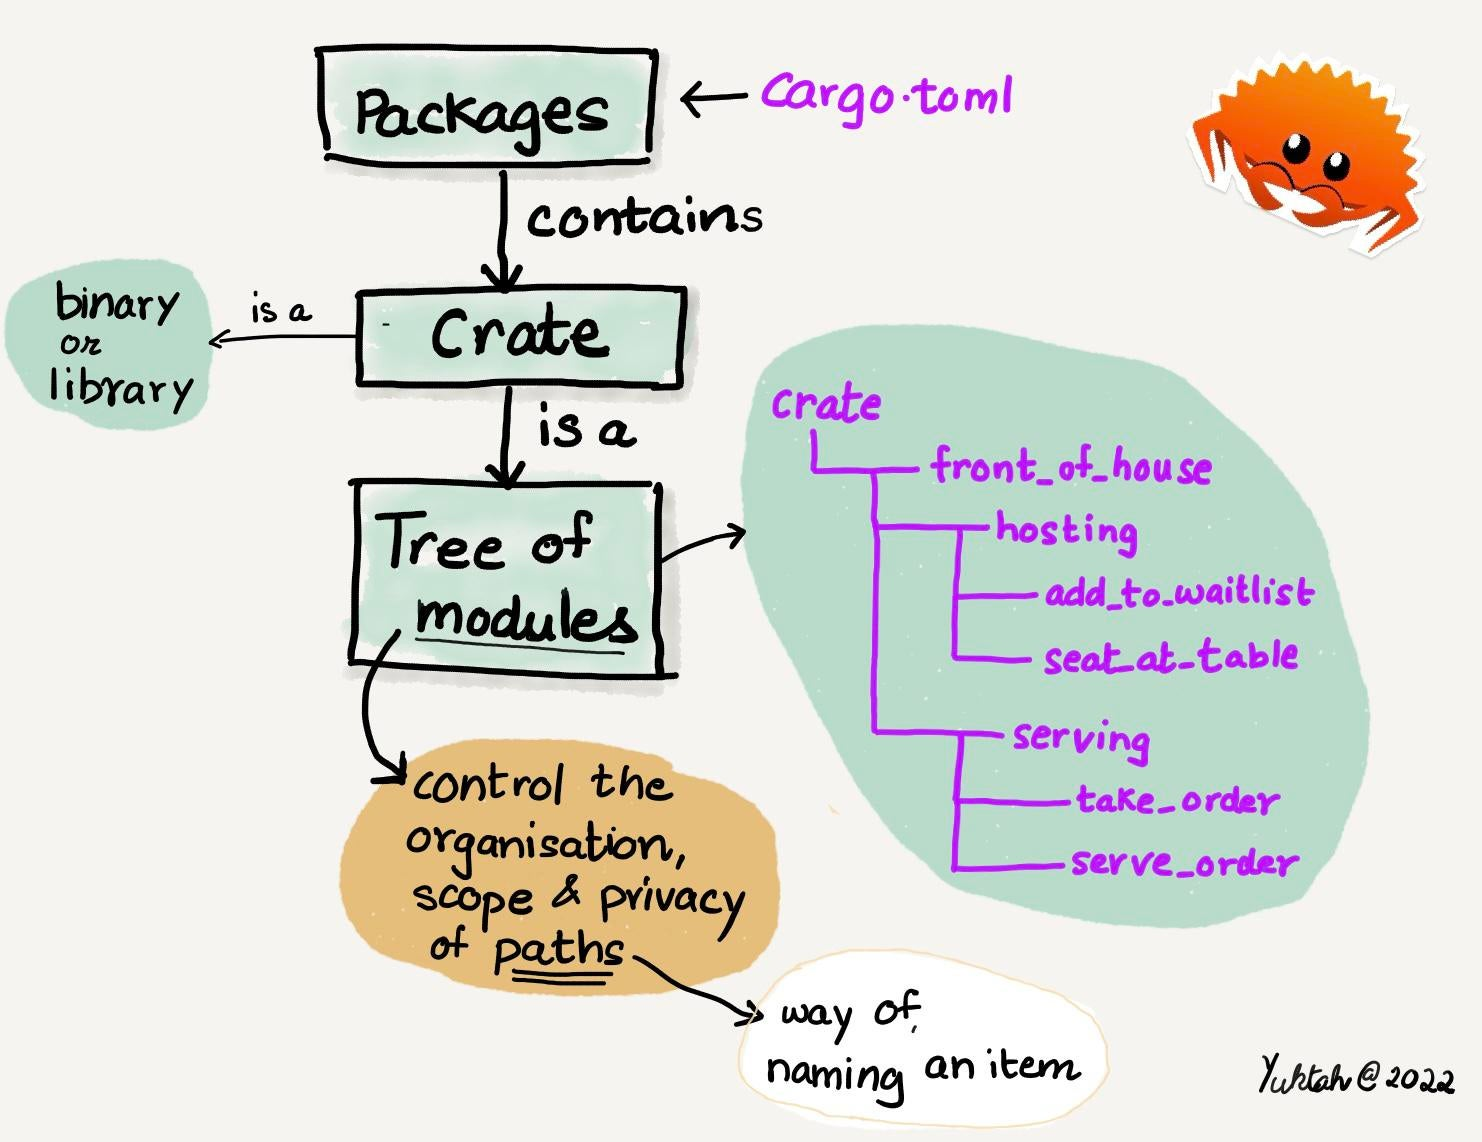
\includegraphics[width=0.65\textwidth]{./img/package.jpeg}
	\end{figure}
\end{frame}

\begin{frame}[fragile]
	\frametitle{Package}
	\begin{itemize}
		\item A package is a bundle of one or more crates that provides a set of functionality. A package contains a Cargo.toml file that describes how to build those crates.
		\item 	After we run \mintinline{shell}|cargo new|, we use \mintinline{shell}|ls| to see what Cargo creates. In the project directory, there’s a \mintinline{shell}|Cargo.toml| file, giving us a package. There’s also a src directory that contains \mintinline{shell}|main.rs|. Cargo knows that if the package directory contains \mintinline{shell}|src/lib.rs|, the package contains a library crate with the same name as the package, and src/lib.rs is its crate root.
		\item If a package contains \mintinline{shell}|src/main.rs| and \mintinline{shell}|src/lib.rs|, it has two crates: a binary and a library, both with the same name as the package. 
	\end{itemize}
\end{frame}

\begin{frame}[fragile]
	\frametitle{Declaring modules}
	In the crate root file, you can \textbf{declare new modules}; say, you declare a “garden” module with  \mintinline{rust}|mod garden;|. The compiler will look for the module’s code in these places:
	\begin{itemize}
		\item 	\textbf{Inline}, within curly brackets that replace the semicolon following \mintinline{rust}|mod garden|
		\item 	\textbf{In the file} src/garden.rs
		\item 	\textbf{In the file} src/garden/mod.rs
	\end{itemize}
	
	\textbf{Declaring submodules}: In any file other than the crate root, you can declare submodules. For example, you might declare \mintinline{rust}|mod vegetables;| in src/garden.rs. The compiler will look for the submodule’s code within the directory named for the parent module in these places:
	\begin{itemize}
		\item 	\textbf{Inline}, directly following mod vegetables, within curly brackets instead of the semicolon
		\item 	\textbf{In the file} src/garden/vegetables.rs
		\item 	\textbf{In the file} src/garden/vegetables/mod.rs
	\end{itemize}
	
\end{frame}


\begin{frame}[fragile]
	\frametitle{Control the privacy with modules}
	\begin{itemize}
		\item Modules let us organize code within a crate for readability and easy reuse. 
		\item 	Modules also\textbf{ allow us to control the privacy of items}, because \textbf{code within a module is private by default}. Private items are internal implementation details not available for outside use.
	\end{itemize}
\end{frame}


\begin{frame}[fragile]
	\frametitle{Paths to code in modules}
	\begin{columns}
		\column{0.3\textwidth}
		Once a module is part of your crate, you can refer to code in that module from anywhere else in that same crate, as long as the privacy rules allow, using the path to the code. For example, an Asparagus type in the garden vegetables module would be found at \mintinline{rust}|crate::garden::vegetables::Asparagus|.
		\column{0.6\textwidth}
		\begin{figure}
			\centering
			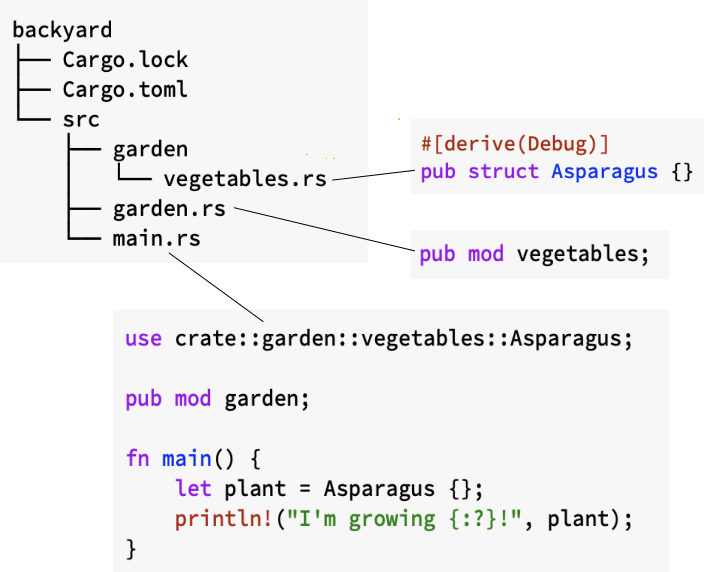
\includegraphics[width=0.9\textwidth]{./img/trpl04-07.png}
		\end{figure}
	\end{columns}
\end{frame}

\begin{frame}[fragile]
	\frametitle{Paths in the Module}
	A path can take two forms:
	
	\begin{itemize}
		\item 	An \textbf{absolute} path is the full path starting from a crate root; for code from an external crate, \textbf{the absolute path begins with the crate name}, and for code from the current crate, it starts with the literal crate.
		\item 	A \textbf{relative} path starts from the current module and \textbf{uses self, super, or an identifier in the current module}.
	\end{itemize}
	Both absolute and relative paths are followed by one or more identifiers separated by double colons (::).
\end{frame}


\begin{frame}[fragile]
	\frametitle{Paths in the Module (2)}
	
	\inputminted{rust}{./code/module.rs}
	
	Both \mintinline{rust}|front_of_house| module and \mintinline{rust}|add_to_waitlist|  method are public. The \mintinline{rust}|pub| keyword lets us use these paths in \mintinline{rust}|add_to_waitlist| with respect to the privacy rules.
\end{frame}

\begin{frame}[fragile]
	\frametitle{Siblings are friend}
	While \mintinline{rust}|front_of_house| isn’t public, because the \mintinline{rust}|eat_at_restaurant| function is defined in the same module as \mintinline{rust}|front_of_house| (that is, \mintinline{rust}|eat_at_restaurant| and \mintinline{rust}|front_of_house| are siblings), we can refer to \mintinline{rust}|front_of_house|  from \mintinline{rust}|eat_at_restaurant|. 
\end{frame}


\begin{frame}[fragile]
	\frametitle{Starting Relative Paths with \mintinline{rust}|super| }
	\inputminted{rust}{./code/module2.rs}
\end{frame}

\begin{frame}[fragile]
	\frametitle{Making Structs Public}
	\inputminted[fontsize=\fontsize{8pt}{8pt}]{rust}{./code/module3.rs}
\end{frame}

\begin{frame}[fragile]
	\frametitle{Making Enums Public}
	\inputminted{rust}{./code/module4.rs}
\end{frame}

\begin{frame}[fragile]
	\frametitle{Bringing Paths into Scope with the \mintinline{rust}|use|  Keyword}
	\begin{itemize}
		\item Having to write out the paths to call functions can feel inconvenient and repetitive. 
		\item 	Fortunately, there’s a way to simplify this process: we can create a shortcut to a path with the use keyword once, and then \mintinline{rust}|use| the shorter name everywhere else in the \textbf{scope}.
	\end{itemize}
	\inputminted{rust}{./code/module5.rs}
	
	Note that  \mintinline{rust}|use| only creates the shortcut for the particular scope in which the use occurs.
\end{frame}


\begin{frame}[fragile]
	\frametitle{Bringing Paths into Scope with the \mintinline{rust}|use|  Keyword (2)}
	\inputminted{rust}{./code/module6.rs}
	To fix this problem, move the \mintinline{rust}|use| within the \mintinline{rust}|customer| module too, or reference the shortcut in the parent module with \mintinline{rust}|super::hosting|  within the child \mintinline{rust}|customer| module.
\end{frame}



\begin{frame}[fragile]
	\frametitle{Creating Idiomatic \mintinline{rust}|use| Paths}
	\inputminted[fontsize=\scriptsize]{rust}{./code/module8.rs}
	
	\inputminted[fontsize=\scriptsize]{rust}{./code/module7.rs}
\end{frame}


\begin{frame}[fragile]
	\frametitle{Creating Idiomatic \mintinline{rust}|use| Paths (2)}
	\begin{itemize}
		\item Bringing the function’s parent module into scope with \mintinline{rust}|use| means we have to specify the parent module when calling the function. \textbf{Specifying the parent module when calling the function makes it clear that the function isn’t locally defined while still minimizing repetition of the full path}. 
		\item On the other hand, when bringing in structs, enums, and other items with use, it’s idiomatic to specify the full path. There’s no strong reason behind this idiom: it’s just the convention that has emerged, and folks have gotten used to reading and writing Rust code this way.
		\inputminted[fontsize=\scriptsize]{rust}{./code/module9.rs}
	\end{itemize}
\end{frame}

\begin{frame}[fragile]
	\frametitle{Creating Idiomatic \mintinline{rust}|use| Paths (3)}
	\inputminted[fontsize=\scriptsize]{rust}{./code/module10.rs}
	
	\begin{block}{Idiomatic way}
		\begin{itemize}
			\item 	\textbf{Function}: bringing the \textbf{function’s parent} module into scope.
			\item 	\textbf{Structs, enums, and other items}: it’s idiomatic to specify the \textbf{full path}.
			\begin{itemize}
				\item The exception to this idiom is if we’re bringing two items with the same name into scope with \mintinline{rust}|use|  statements, because Rust doesn’t allow that.
			\end{itemize}
		\end{itemize}
	\end{block}
	
\end{frame}



\begin{frame}[fragile]
	\frametitle{Providing New Names with the as Keyword}
	\inputminted[fontsize=\scriptsize]{rust}{./code/module11.rs}
\end{frame}



\begin{frame}[fragile]
	\frametitle{Re-exporting Names with \mintinline{rust}|pub use|}
	When we bring a name into scope with the use keyword, the name available in the new scope is private. To enable the code that calls our code to refer to that name as if it had been defined in that code’s scope, we can combine  \mintinline{rust}|pub| and  \mintinline{rust}|use|.
	
	\inputminted[fontsize=\scriptsize]{rust}{./code/module12.rs}
	
	\scriptsize
	It makes our library well organized for programmers working on the library and programmers calling the library. 
\end{frame}



\begin{frame}[fragile]
	\frametitle{Using External Packages}
	Members of the Rust community have made many packages available at \url{crates.io}, and pulling any of them into your package involves these same steps: listing them in your package’s \mintinline{rust}|Cargo.toml| file and using use to bring items from their crates into scope. Example:
	
	1) Add the following line to \mintinline{rust}|Cargo.toml| file.
	
	\mintinline{toml}|rand = "0.8.5"|
	
	2) bring items from the crates into scope (with \mintinline{rust}|use|) and used it.
	\inputminted{rust}{./code/module13.rs}
\end{frame}


\begin{frame}[fragile]
	\frametitle{Using Nested Paths to Clean Up Large \mintinline{rust}|use| Lists}
	\inputminted{rust}{./code/module14.rs}
\end{frame}


\begin{frame}[fragile]
	\frametitle{Separating Modules into Different Files}
	\begin{itemize}
		\item For a module named  \mintinline{rust}|front_of_house| declared in the crate root, the compiler will look for the module’s code in:
		\begin{itemize}
			\item \mintinline{rust}|src/front_of_house.rs| (what we covered)
			\item 	\mintinline{rust}|src/front_of_house/mod.rs| (older style, still supported path)
		\end{itemize}
		\item 	For a module named hosting that is a submodule of \mintinline{rust}|front_of_house| , the compiler will look for the module’s code in:
		\begin{itemize}
			\item \mintinline{rust}|src/front_of_house/hosting.rs| (what we covered)
			\item 	\mintinline{rust}|src/front_of_house/hosting/mod.rs| (older style, still supported path)
		\end{itemize}
		\item 	If you use both styles for the same module, you’ll get a compiler error. Using a mix of both styles for different modules in the same project is allowed, but might be confusing for people navigating your project.
		\item The main downside to the style that uses files named mod.rs is that your project can end up with many files named mod.rs, which is confusing.
	\end{itemize}
	
\end{frame}

\section{Common Collections}
\begin{frame}[fragile]
	\frametitle{Collections}
	\begin{itemize}
		\item \textbf{Rust’s standard library} includes a number of very useful \textbf{data structures} called \textbf{collections}. 
		\item 	Most other data types represent one specific value, but collections can contain multiple values. 
		\item 	Unlike the built-in array and tuple types, the data these collections point to is stored on the \textbf{heap}, which means the amount of data does not need to be known at compile time and can grow or shrink as the program runs.
		\item 	Each kind of collection has different capabilities and costs, and choosing an appropriate one for your current situation is a skill you’ll develop over time. 
		\item Rust’s collections can be grouped into four major categories:
		\begin{itemize}
			\item 	\textbf{Sequences}: Vec, VecDeque(double-ended queue), LinkedList
			\item 	\textbf{Maps}: HashMap, BTreeMap
			\item 	\textbf{Sets}: HashSet, BTreeSet
			\item 	\textbf{Misc}: BinaryHeap
		\end{itemize}
	\end{itemize}
\end{frame}

\begin{frame}[fragile]
	\frametitle{Creating a New Vector}
	\inputminted{rust}{./code/vector.rs}
\end{frame}

\begin{frame}[fragile]
	\frametitle{Reading Elements of Vectors}
	There are two ways to reference a value stored in a vector: via indexing or using the get method. 
	
	\inputminted[fontsize=\scriptsize]{rust}{./code/vector2.rs}
	
	The reason Rust provides these two ways to reference an element is so you can choose how the program behaves when you try to use an index value outside the range of existing elements.
\end{frame}


\begin{frame}[fragile]
	\frametitle{Iterating over the Values in a Vector}
	\inputminted{rust}{./code/vector3.rs}
\end{frame}

\begin{frame}[fragile]
	\frametitle{Using an Enum to Store Multiple Types}
	\inputminted{rust}{./code/vector4.rs}
\end{frame}

\begin{frame}[fragile]
	\frametitle{Using an Enum to Store Multiple Types}
	\inputminted{rust}{./code/vector4.rs}
\end{frame}

\begin{frame}[fragile]
	\frametitle{What Is a \mintinline{rust}|String|?}
	
	\begin{itemize}
		\item 	Many of the same operations available with \mintinline{rust}|Vec<T>|  are available with \mintinline{rust}|String| as well, because String is actually implemented as a wrapper around \textbf{a vector of bytes} with some extra guarantees, restrictions, and capabilities.
		\item 	Rust has only one \textbf{string type}\textit{ in the core language}, which is the \textbf{string slice} \mintinline{rust}|str| that is usually seen in its borrowed form \mintinline{rust}|&str|. 
		\item 	The \textbf{String type}, which is provided by\textbf{ Rust’s standard library} rather than coded into the core language, is \textit{a growable, mutable, owned, UTF-8 encoded string type}. When Rustaceans refer to “strings” in Rust, they might be referring to either the String or the string slice \mintinline{rust}|&str| types, not just one of those types. 
	\end{itemize}
\end{frame}


\begin{frame}[fragile]
	\frametitle{Creating a New String}
	\inputminted{rust}{./code/string_vec.rs}
	
	Because strings are used for so many things, we can use many different generic APIs for strings, providing us with a lot of options. Some of them can seem redundant, but they all have their place! In this case, \mintinline{rust}|String::from| and \mintinline{rust}|to_string| do the same thing, so which you choose is a matter of style and readability.
\end{frame}


\begin{frame}[fragile]
	\frametitle{Updating a String}
	\inputminted{rust}{./code/string_vec2.rs}
\end{frame}

\begin{frame}[fragile]
	\frametitle{Hash Maps}
	\inputminted{rust}{./code/map.rs}
\end{frame}


\begin{frame}[fragile]
	\frametitle{Hash Maps and Ownership}
	For types that implement the Copy trait, like i32, the values are copied into the hash map. For owned values like String, the values will be moved and the hash map will be the owner of those values.
	
	\inputminted{rust}{./code/map2.rs}
\end{frame}

\section{Error Handling}

\begin{frame}[fragile]
	\frametitle{Rust errors categories}
	Rust groups errors into two major categories: \textbf{recoverable} and \textbf{unrecoverable} errors. 
	\begin{itemize}
		\item For a \textbf{recoverable} error, such as a file not found error, we most likely just want to report the problem to the user and retry the operation. 
		\item 	\textbf{Unrecoverable} errors are always \textbf{symptoms of bugs}, like trying to access a location beyond the end of an array, and so we want to immediately \textbf{stop the program}.
		\item  Rust doesn’t have exceptions. Instead, it has the type \mintinline{rust}|Result<T, E>| for recoverable errors and the  \mintinline{rust}|panic!| macro that stops execution when the program encounters an unrecoverable error.
	\end{itemize}
	
\end{frame}

\begin{frame}[fragile]
	\frametitle{Unrecoverable Errors with panic!}
	\inputminted{rust}{./code/panic.rs}
	
	\begin{block}{Unwinding the Stack }
		By default, when a panic occurs, the program starts unwinding, which means Rust walks back up the stack and cleans up the data from each function it encounters. However, this walking back and cleanup is a lot of work. Rust, therefore, allows you to choose the alternative of immediately aborting, which ends the program without cleaning up.
	\end{block}
\end{frame}


\begin{frame}[fragile]
	\frametitle{Recoverable Errors with Result}
	Most errors aren’t serious enough to require the program to stop entirely. Sometimes, when a function fails, it’s for a reason that you can easily interpret and respond to (For example, open a file that doesn’t exist).
	
	\scriptsize
	
	\inputminted[fontsize=\scriptsize]{rust}{./code/result.rs}
	
	\inputminted[fontsize=\scriptsize]{rust}{./code/result2.rs}
\end{frame}


\begin{frame}[fragile]
	\frametitle{Matching on Different Errors}
	
	\inputminted[fontsize=\scriptsize]{rust}{./code/result3.rs}
\end{frame}


\begin{frame}[fragile]
	\frametitle{Alternatives to Using match with \mintinline{rust}|Result<T, E>| }
	
	\inputminted[fontsize=\scriptsize]{rust}{./code/result4.rs}
\end{frame}

\begin{frame}[fragile]
	\frametitle{Shortcuts for Panic on Error: unwrap and expect }
	\scriptsize
	The \mintinline{rust}|Result<T, E>| type has many helper methods defined on it to do various, more specific tasks. If the Result value is the Ok variant, unwrap will return the value inside the Ok. If the Result is the Err variant, unwrap will call the panic! macro for us.
	
	\inputminted[fontsize=\scriptsize]{rust}{./code/result5.rs}
	
	We use  \mintinline{rust}|expect| in the same way as unwrap: to return the file handle or call the panic! macro.
	
	\inputminted[fontsize=\scriptsize]{rust}{./code/result6.rs}
\end{frame}



\begin{frame}[fragile]
	\frametitle{Propagating Errors with  \mintinline{rust}|?| Operator}
	\inputminted{rust}{./code/result8.rs}
\end{frame}

\begin{frame}[fragile]
	\frametitle{A Shortcut for Propagating Errors: the \mintinline{rust}|?| Operator}
	\inputminted{rust}{./code/result7.rs}
\end{frame}

\begin{frame}[fragile]
	\frametitle{A Shortcut for Propagating Errors: the \mintinline{rust}|?| Operator}
	\inputminted[fontsize=\scriptsize]{rust}{./code/result9.rs}
	
	\inputminted[fontsize=\scriptsize]{rust}{./code/result10.rs}
\end{frame}

\begin{frame}[fragile]
	\frametitle{Where The \mintinline{rust}|?| Operator Can Be Used}
	\begin{itemize}
		\item 	The \mintinline{rust}|?| operator can only be used in functions whose return type is compatible with the value the \mintinline{rust}|?| is used on.
		\item 	we’re only allowed to use the ? operator in a function that returns \mintinline{rust}|Result|, \mintinline{rust}|Option|, or another type that implements \mintinline{rust}|FromResidual|.
	\end{itemize}
	
	\inputminted{rust}{./code/result11.rs}
\end{frame}

\begin{frame}[fragile]
	\frametitle{Where The \mintinline{rust}|?| Operator Can Be Used (2)}
	\inputminted{rust}{./code/result12.rs}
	
	The \mintinline{rust}| Box<dyn Error>| type is a trait object, which we’ll talk about later. For now, you can read \mintinline{rust}| Box<dyn Error>|  to mean “any kind of error.” 
	
\end{frame}

\section{Generic Types, Traits, and Lifetimes}

\begin{frame}[fragile]
	\frametitle{Generic Data Types}
	We use generics to create definitions for items like function signatures or structs, which we can then use with many different concrete data types.
	
	\begin{columns}
		\column{0.5\textwidth}
		\inputminted{rust}{./code/generic1.rs}
		\column{0.5\textwidth}
		\inputminted{rust}{./code/generic2.rs}
	\end{columns}
\end{frame}

\begin{frame}[fragile]
	\frametitle{Generic Data Types (3)}
	\inputminted[fontsize=\scriptsize]{rust}{./code/generic3.rs}
\end{frame}

\begin{frame}[fragile]
	\frametitle{Generic Data Types In Struct Definitions}
	\inputminted{rust}{./code/generic4.rs}
\end{frame}

\begin{frame}[fragile]
	\frametitle{Generic Data Types In Enum Definitions}
	\inputminted{rust}{./code/generic5.rs}
\end{frame}


\begin{frame}[fragile]
	\frametitle{Generic Data Types In Method Definitions}
	\inputminted[fontsize=\scriptsize]{rust}{./code/generic6.rs}
\end{frame}

\begin{frame}[fragile]
	\frametitle{Generic Data Types In Method Definitions(2)}
	\inputminted[fontsize=\scriptsize]{rust}{./code/generic7.rs}
\end{frame}


\begin{frame}[fragile]
	\frametitle{Monomorphization}
	Monomorphization is the process of turning generic code into specific code by filling in the concrete types that are used when \textbf{compiled}. In this process, the compiler does the opposite of the steps we used to create the generic function: the compiler looks at all the places where generic code is called and generates code for the concrete types the generic code is called with.
	
\end{frame}

\begin{frame}[fragile]
	\frametitle{Monomorphization}
	
	\inputminted[fontsize=\scriptsize]{rust}{./code/generic8.rs}
\end{frame}


\begin{frame}[fragile]
	\frametitle{Traits: Defining Shared Behavior}
	\begin{itemize}
		\item A trait defines functionality a particular type has and can share with other types. We can use traits \textbf{to define shared behavior in an abstract way}. We can use trait bounds to specify that a generic type can be any type that has certain behavior.
		\item 	Note: Traits are similar to a feature often called \textbf{interfaces in other languages}, although with some differences.
		\item 	Trait definitions are a way to group method signatures together to define a set of behaviors necessary to accomplish some purpose.
	\end{itemize}
\end{frame}


\begin{frame}[fragile]
	\frametitle{Traits: Defining Shared Behavior (2)}
	\inputminted[fontsize=\scriptsize]{rust}{./code/Trait1.rs}
\end{frame}


\begin{frame}[fragile]
	\frametitle{Traits: Default Implementations}
	\inputminted[fontsize=\scriptsize]{rust}{./code/Trait2.rs}
\end{frame}


\begin{frame}[fragile]
	\frametitle{Traits as Parameters}
	\inputminted{rust}{./code/Trait3.rs}
\end{frame}



\begin{frame}[fragile]
	\frametitle{Clearer Trait Bounds with where Clauses}
	A functions with multiple generic type parameters can contain lots of trait bound information between the function’s name and its parameter list, making the function signature hard to read. For this reason, Rust has alternate syntax for specifying trait bounds inside a where clause after the function signature. So instead of writing this:
	
	\inputminted[fontsize=\scriptsize]{rust}{./code/trait4.rs}
	
	we can use a where clause, like this:
	
	\inputminted[fontsize=\scriptsize]{rust}{./code/trait5.rs}
\end{frame}

\begin{frame}[fragile]
	\frametitle{Validating References with Lifetimes}
	\begin{itemize}
		\item lifetimes \textbf{ensure that references are valid as long as we need them to be}.
		\item 	Lifetimes are another \textbf{kind of generic} that we’ve already been using.
		\item 	Most of the time, lifetimes are implicit and inferred, just like most of the time, types are inferred. We only must annotate types when multiple types are possible.
		\item 	Annotating lifetimes is not even a concept most other programming languages have, so this is going to feel \textbf{unfamiliar}.
		\item The Rust compiler has a\textbf{ borrow checker} that compares scopes to determine whether all borrows are valid.
		\begin{itemize}
			\item borrowing: the action of creating a reference.
		\end{itemize}
	\end{itemize}
\end{frame}

\begin{frame}[fragile]
	\frametitle{Preventing Dangling References with Lifetimes}
	Annotations of the lifetimes of r and x, named 'a and 'b, respectively
	
	\inputminted{rust}{./code/dangling-ref.rs}
	
	The variable x doesn’t “live long enough.” The reason is that x will be out of scope when the inner scope ends on line 7. But r is still valid for the outer scope; because its scope is larger, we say that it “lives longer.” 
\end{frame}

\begin{frame}[fragile]
	\frametitle{Preventing Dangling References with Lifetimes(2)}
	\inputminted{shell}{./code/dangling-ref.shell}
\end{frame}


\begin{frame}[fragile]
	\frametitle{Generic Lifetimes in Functions}
	We’ll write a function that returns the longer of two string slices. This function will take two string slices and return a single string slice.
	
	\inputminted{rust}{./code/lifetime.rs}
\end{frame}



\begin{frame}[fragile]
	\frametitle{Generic Lifetimes in Functions (2)}
	Rust can’t tell whether the reference being returned refers to x or y. Actually, we don’t know either, because the if block in the body of this function returns a reference to x and the else block returns a reference to y!
	
	\inputminted{rust}{./code/lifetime2.rs}
\end{frame}


\begin{frame}[fragile]
	\frametitle{Generic Lifetimes in Functions (3)}
	\inputminted{shell}{./code/lifetime2.shell}
\end{frame}

\begin{frame}[fragile]
	\frametitle{Lifetime Annotation Syntax}
	\begin{itemize}
		\item 	Lifetime annotations \textbf{don’t change how long any of the references live}. Rather, they \textbf{describe the relationships of the lifetimes of multiple references to each other }without affecting the lifetimes.
		\item 	Lifetime annotations have a slightly \textbf{unusual syntax}: the names of lifetime parameters must start with an apostrophe (') and are usually all lowercase and very short, like generic types. Most people use the name \mintinline{rust}|'a| for the first lifetime annotation. We place lifetime parameter annotations after the \mintinline{rust}|&| of a reference, using a space to separate the annotation from the reference’s type.
		
		\inputminted{rust}{./code/lifetime3.rs}
	\end{itemize}
\end{frame}


\begin{frame}[fragile]
	\frametitle{Lifetime Annotations in Function Signatures}
	\inputminted{rust}{./code/lifetime4.rs}
	
	The generic lifetime \mintinline{rust}|'a| will get the concrete \textbf{lifetime that is equal to the smaller of the lifetimes }of x and y. In practice, it means that the lifetime of the reference returned by the longest function is the same as the smaller of the lifetimes of the values referred to by the function arguments. These relationships are what we want Rust to use when analyzing this code.
\end{frame}


\begin{frame}[fragile]
	\frametitle{Lifetime Annotations in Function Signatures (2)}
	\inputminted{rust}{./code/lifetime5.rs}
	
	The error shows that for result to be valid for the \mintinline{rust}|println!| statement, string2 would need to be valid until the end of the outer scope. Rust knows this because we annotated the lifetimes of the function parameters and return values using the same lifetime parameter \mintinline{rust}|'a|.
	
\end{frame}

\begin{frame}[fragile]
	\frametitle{Lifetime Annotations in Function Signatures (3)}
	\inputminted{shell}{./code/lifetime5.shell}
	
\end{frame}

\begin{frame}[fragile]
	\frametitle{Lifetime Annotations in Struct Definitions}
	\inputminted{rust}{./code/lifetime6.rs}
	
	We can define structs to hold references, but in that case we would need to add a lifetime annotation on every reference in the struct’s definition.
	
\end{frame}

\begin{frame}[fragile]
	\frametitle{Lifetime Elision}
	\begin{itemize}
		\item In early versions (pre-1.0) of Rust, every reference needed an explicit lifetime. After writing a lot of Rust code, the Rust team found that Rust programmers were entering the same lifetime annotations over and over in particular situations. These situations were predictable and followed a few deterministic patterns. After writing a lot of Rust code, the Rust team found that Rust programmers were entering \textbf{the same lifetime annotations over and over in particular situations. These situations were predictable and followed a few deterministic patterns}. 
		\item  \textbf{The patterns programmed into Rust’s analysis of references are called thelifetime elision} rules. These aren’t rules for programmers to follow; they’re a set of particular cases that the compiler will consider, and if your code fits these cases, you don’t need to write the lifetimes explicitly.
	\end{itemize}
	
\end{frame}


\begin{frame}[fragile]
	\frametitle{Lifetime Elision (2)}
	\begin{itemize}
		\item The first rule is that the compiler assigns a lifetime parameter to each parameter that’s a reference. In other words, a function with one parameter gets one lifetime parameter: \mintinline{rust}|fn foo<'a>(x: &'a i32);|  a function with two parameters gets two separate lifetime parameters: \mintinline{rust}|fn foo<'a, 'b>(x: &'a i32, y: &'b i32);| and so on.
		\item 	The second rule is that, if there is exactly one input lifetime parameter, that lifetime is assigned to all output lifetime parameters: \mintinline{rust}|fn foo<'a>(x: &'a i32) -> &'a i32|.
		\item 	The third rule is that, if there are multiple input lifetime parameters, but one of them is \mintinline{rust}|&self| or \mintinline{rust}|&mut self| because this is a method, the lifetime of \mintinline{rust}|self| is assigned to all output lifetime parameters. This third rule makes methods much nicer to read and write because fewer symbols are necessary.
	\end{itemize}
	
\end{frame}

\begin{frame}[fragile]
	\frametitle{Lifetime Elision (2)}
	
	\inputminted[fontsize=\scriptsize]{rust}{./code/lifetime7.rs}
\end{frame}


\begin{frame}[fragile]
	\frametitle{Lifetime Annotations in Method Definitions}
	When we implement methods on a struct with lifetimes, we use the same syntax as that of generic type parameters shown: 
	
	\inputminted{rust}{./code/lifetime8.rs}
	
	The lifetime parameter declaration after impl and its use after the type name are required, but we’re not required to annotate the lifetime of the reference to self because of the first elision rule.
\end{frame}

\begin{frame}[fragile]
	\frametitle{The Static Lifetime}
	One special lifetime we need to discuss is \mintinline{rust}|'static|, which denotes that the affected reference can live for the entire duration of the program. All string literals have the \mintinline{rust}|'static| lifetime, which we can annotate as follows:
	
	\inputminted{rust}{./code/lifetime9.rs}
	
	The text of this string is stored directly in the program’s binary, which is always available. Therefore, the lifetime of all string literals is 'static.
\end{frame}


\begin{frame}[fragile]
	\frametitle{Generic Type Parameters, Trait Bounds, and Lifetimes Together}
	
	\inputminted{rust}{./code/lifetime10.rs}
\end{frame}

\section{Writing Automated Tests}

\begin{frame}[fragile]
	\frametitle{The Anatomy of a Test Function}
	
	\inputminted{rust}{./code/test1.rs}
	
	\inputminted[fontsize=\scriptsize]{shell}{./code/test1.shell}
\end{frame}

\begin{frame}[fragile]
	\frametitle{ Adding a second test that will fail because we call the \mintinline{rust}|panic!| macro}
	
	\inputminted{rust}{./code/test2.rs}
\end{frame}


\begin{frame}[fragile]
	\frametitle{Checking Results with the  \mintinline{rust}|assert!| Macro}
	The \mintinline{rust}|assert!| macro, provided by the standard library, is useful when you want to ensure that some condition in a test evaluates to true. 
	
	\inputminted[fontsize=\scriptsize]{rust}{./code/test3.rs}
\end{frame}

\begin{frame}[fragile]
	\frametitle{Checking Results with the \mintinline{rust}|assert_eq!| and \mintinline{rust}|assert_ne!| Macro}
	
	\inputminted{rust}{./code/test4.rs}
\end{frame}

\begin{frame}[fragile]
	\frametitle{Adding Custom Failure Messages}
	You can also add a custom message to be printed with the failure message as optional arguments to the \mintinline{rust}|assert!|, \mintinline{rust}|assert_eq!|, and \mintinline{rust}|assert_ne!| macros. Any arguments specified after the required arguments are passed along to the \mintinline{rust}|format!| macro
	
	\inputminted[fontsize=\scriptsize]{rust}{./code/test5.rs}
\end{frame}



\begin{frame}[fragile]
	\frametitle{Checking for Panics with \mintinline{rust}|should_panic|}
	
	\inputminted[fontsize=\scriptsize]{rust}{./code/test6.rs}
\end{frame}



\begin{frame}[fragile]
	\frametitle{Using \mintinline{rust}|Result<T, E>| in Tests}
	
	\inputminted{rust}{./code/test7.rs}
	
	Writing tests so they return a \mintinline{rust}|Result<T, E>| enables you to use the question mark operator in the body of tests, which can be a convenient way to write tests that should fail if any operation within them returns an Err variant.
	
\end{frame}


\begin{frame}[fragile]
	\frametitle{Controlling How Tests Are Run}
	\begin{itemize}
		\item \mintinline{shell}|cargo test| compiles your code in test mode and runs the resulting test binary. The default behavior of the binary produced by cargo test is to \textbf{run all the tests in parallel} and capture output generated during test runs,\textbf{ preventing the output from being displayed} and making it easier to read the output related to the test results. You can, however, specify command line options to change this default behavior.
		\item If you don’t want to run the tests in parallel or if you want more fine-grained control over the number of threads used, you can send the \mintinline{shell}|--test-threads|  flag and the number of threads you want to use to the test binary (ex: \mintinline{shell}|cargo test -- --test-threads=1| ).
		\item If we call \mintinline{rust}|println!|  in a test, we won’t see the \mintinline{rust}|println!| output in the terminal. If we want to see printed values for passing tests, we can tell Rust to also show the output of successful tests with \mintinline{shell}|cargo test -- --show-output|.
	\end{itemize}
\end{frame}

\begin{frame}[fragile]
	\frametitle{Controlling How Tests Are Run(2)}
	\begin{itemize}
		\item Sometimes, running a full test suite can take a long time:
		\begin{itemize}
			\item If we run the tests without passing any arguments, all the tests will run in parallel
			\item 	We can pass the name of any test function to  \mintinline{shell}|cargo test| to run only that test.
			\item 	We can specify part of a test name, and any test whose name matches that value will be run.
		\end{itemize}
		\item Sometimes a few specific tests can be very time-consuming to execute, so you might want to exclude them during most runs of \mintinline{shell}|cargo test|. After  \mintinline{shell}|#[test]| we add the  \mintinline{shell}|#[ignore]| line to the test we want to exclude.   If we want to run only the ignored tests, we can use  \mintinline{shell}|cargo test -- --ignored|.
		\inputminted[fontsize=\scriptsize]{rust}{./code/test8.rs}
	\end{itemize}
\end{frame}



\begin{frame}[fragile]
	\frametitle{Test Organization}
	\begin{itemize}
		\item The Rust community thinks about tests in terms of two main categories: \textbf{unit tests} and \textbf{integration tests}. 
		\begin{itemize}
			\item Unit tests are small and more focused, \textbf{testing one module in isolation at a time}, and \textbf{can test private interfaces}.  You’ll put unit tests in the \mintinline{shell}|src| directory in each file with the code that they’re testing. The convention is to create a module named tests in each file to contain the test functions and to annotate the module with \mintinline{rust}|#[cfg(test)]|.
			\item Integration tests are entirely external to your library and use your code in the same way any other external code would,\textbf{ using only the public interface and potentially exercising multiple modules per test}. Their purpose is to test \textbf{whether many parts of your library work together correctly}.
		\end{itemize}
	\end{itemize}
\end{frame}


\begin{frame}[fragile]
	\frametitle{Integration test}
	We create a tests directory at the top level of our project directory, next to src. Cargo knows to look for integration test files in this directory. We can then make as many test files as we want, and Cargo will compile each of the files as an individual crate.
	
	
	\begin{columns}
		\column{0.4\textwidth}
		\begin{figure}
			\centering
			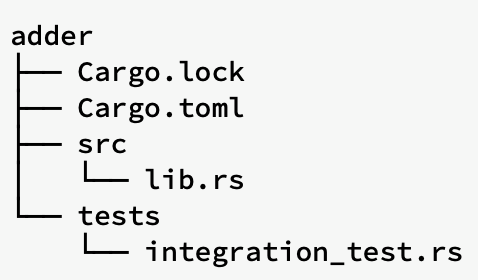
\includegraphics[width=0.8\linewidth]{img/test.png}
		\end{figure}
		\column{0.6\textwidth}
		\scriptsize
		Filename: \mintinline{shell}|tests/integration_test.rs|
		\inputminted[fontsize=\scriptsize]{rust}{./code/test9.rs}
		
		\mintinline{shell}|$ cargo test|
		
		\mintinline{shell}|$ cargo test --test integration_test|
	\end{columns}
\end{frame}



\begin{frame}[fragile]
	\frametitle{Submodules in Integration Tests}
	For example, if we create \mintinline{shell}|tests/common.rs| and place a function named setup in it, we can add some code to \mintinline{rust}|tsetup| that we want to call from multiple test functions in multiple test files:
	
	
	\begin{columns}
		\column{0.4\textwidth}
		\begin{figure}
			\centering
			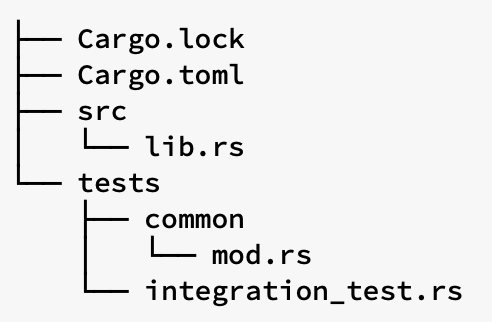
\includegraphics[width=0.8\linewidth]{img/test2.png}
		\end{figure}
		\column{0.6\textwidth}
		\scriptsize
		Filename: \mintinline{shell}|tests/common.rs|
		\inputminted[fontsize=\scriptsize]{rust}{./code/test10.rs}
	\end{columns}
	\scriptsize
	Filename: \mintinline{shell}|tests/integration_test.rs|
	
	\inputminted[fontsize=\scriptsize]{rust}{./code/test11.rs}
	
\end{frame}

\section{An I/O Project: Building a Command Line Program}


\begin{frame}[fragile]
	\frametitle{minigrep example}
	\begin{itemize}
		\item 	We’ll make our own version of the classic command line search tool grep (globally search a regular expression and print). In the simplest use case, grep searches a specified file for a specified string. 
		\item 	The first task is to make \textbf{minigrep} accept its two command line arguments: the \textbf{file path} and \textbf{a string to search for}. That is, we want to be able to run our program with cargo run, \textbf{two hyphens to indicate the following arguments are for our program rather than for cargo}, a string to search for, and a path to a file to search in, like so: \mintinline{shell}|$ cargo run -- searchstring example-filename.txt|
	\end{itemize}
	
\end{frame}

\begin{frame}[fragile]
	\frametitle{minigrep - Reading the Argument Values}
	\inputminted[fontsize=\scriptsize]{rust}{./code/grep1.rs}
	
	\inputminted[fontsize=\scriptsize]{shell}{./code/grep1.shell}
	
	Notice that the first value in the vector is the name of our binary.
\end{frame}

\begin{frame}[fragile]
	\frametitle{minigrep - Saving the Argument Values in Variables}
	\inputminted[fontsize=\scriptsize]{rust}{./code/grep2.rs}
\end{frame}


\section{Functional Language Features: Iterators and Closures}

\section{More About Cargo and Crates.io}
\section{Smart Pointers}
\section{Fearless Concurrency}
\section{Object-Oriented Programming Features of Rust}
\section{Patterns and Matching}
\section{Advanced Features}
\section{Multithread Web Server}
\section{Tokio}

\section*{Acknowledgement}
\begin{frame}
	\Huge{\centerline{Thank you!}}
\end{frame}

\end{document}

\begin{comment}
\begin{frame}[fragile]
	\frametitle{title}
\end{frame}

\begin{columns}
	\column{0.5\textwidth}
	\tableofcontents[sections = 1-10]
	\column{0.5\textwidth}
	\tableofcontents[sections = 11-20]
\end{columns}
\end{comment}
